% Sostituisco i placeholder registrati con la specifica variabile per il documento corrente. Questa parte iniziale contiene intestazioni e templates.

% Modificare ad ogni modifica e documento1
\newcommand{\documento}{Manuale Manutentore}
\newcommand{\nomedocumentofisico}{ManualeManutentore 1\_0\_0.pdf}
\newcommand{\redazione}{\MC \\ & \DAN \\ & \DS \\ & \AN}
\newcommand{\verifica}{\AS \\ & \NS}
\newcommand{\versione}{1.0.0}
\newcommand{\approvazione}{\DAN}
\newcommand{\uso}{Esterno}
\newcommand{\destinateTo}{\TV, \\ & \RC, \\ & \gruppo}
\newcommand{\datacreazione}{15 maggio 2017}
\newcommand{\datamodifica}{17 giugno 2017}
\newcommand{\stato}{Approvato}

%Abilitazione indice delle tabelle e figure
\def\TABELLE{false}
\def\FIGURE{false}

%Inclusione di layout e variabili (Non modificare)
%Stile e dimensione del documento
\documentclass[a4paper,11pt]{article}

%Pacchetti da importare
\usepackage{ifthen}
\usepackage[italian]{babel}
\usepackage[utf8]{inputenc}
\usepackage[T1]{fontenc}
\usepackage{float}
\usepackage{chapterbib}
\usepackage{graphicx}
\usepackage[a4paper,top=2.5cm,bottom=2.5cm,left=2.5cm,right=2.5cm]{geometry}
\usepackage[colorlinks=true, urlcolor=black, citecolor=black, linkcolor=black]{hyperref}
\usepackage{booktabs}
\usepackage{fancyhdr}
\usepackage{totpages}
\usepackage{tabularx, array}
\usepackage{dcolumn}
\usepackage{epstopdf}
\usepackage{booktabs}
\usepackage{fancyhdr}
\usepackage{longtable}
\usepackage{calc}
\usepackage{datatool}
\usepackage[bottom]{footmisc}
\usepackage{listings}
\usepackage{textcomp}
\usepackage{titlesec}
\usepackage{rotating}
\usepackage{multirow}
\usepackage{placeins}
\usepackage{color}
\usepackage[table,usenames,dvipsnames]{xcolor}
\usepackage{hyperref}
\usepackage{makecell}
\usepackage{breakurl}
\usepackage{hyperref}
\usepackage{multirow}
\usepackage{xcolor,colortbl}
\usepackage{afterpage}
\usepackage{mathtools}
\usepackage{verbatim} 
\usepackage[toc,page]{appendix}

%glossary code%
\usepackage[nonumberlist,xindy]{glossaries}

\newglossarystyle{myaltlistgroup}{%
	\setglossarystyle{altlistgroup}%
	\renewcommand*{\glsgroupheading}[1]{%
		
		\newpage
		\item\makebox[\linewidth]{\Large\textbf{\glsgetgrouptitle{##1}}}%
		\vspace*{-\baselineskip}%
		\item\makebox[\linewidth]{\hspace*{3cm}\hrulefill\hspace*{3cm}}%
	}%
}



%Stile fancy per il documento (Header e footer)
\pagestyle{fancy}
%Rimuovo l'indentazione
\setlength{\parindent}{0pt}

%Imposto l'intestazione
\lhead{\Large{\progetto} \\ \footnotesize{\documento}}
%Linea sotto l'intestazione
\renewcommand{\headrulewidth}{0.4pt} 

%Footer
\lfoot{\textit{\gruppoLink}\\ \footnotesize{\email}}
%Footer con numero romano per le prime pagine
\rfoot{\thepage}
\cfoot{}
%Linea sopra il footer
\renewcommand{\footrulewidth}{0.4pt}   

%Imposta il livello degli elenchi 
\setcounter{secnumdepth}{7}
\setcounter{tocdepth}{7}

%Paragrafi impostati come una sezione
\titleformat{\paragraph}{\normalfont\normalsize\bfseries}{\theparagraph}{1em}{}
\titlespacing*{\paragraph}{0pt}{3.25ex plus 1ex minus .2ex}{1.5ex plus .2ex}

\titleformat{\subparagraph}{\normalfont\normalsize\bfseries}{\thesubparagraph}{1em}{}
\titlespacing*{\subparagraph}{0pt}{3.25ex plus 1ex minus .2ex}{1.5ex plus .2ex}

\makeatletter
\newcounter{subsubparagraph}[subparagraph]
\renewcommand\thesubsubparagraph{
  \thesubparagraph.\@arabic\c@subsubparagraph}
\newcommand\subsubparagraph{
  \@startsection{subsubparagraph}
    {6}
    {\parindent}
    {3.25ex \@plus 1ex \@minus .2ex}
    {0.75em}
    {\normalfont\normalsize\bfseries}}
\newcommand\l@subsubparagraph{\@dottedtocline{6}{10em}{5.5em}} 
\newcommand{\subsubparagraphmark}[1]{}
\makeatother

\makeatletter
\newcounter{subsubsubparagraph}[subsubparagraph]
\renewcommand\thesubsubsubparagraph{
  \thesubsubparagraph.\@arabic\c@subsubsubparagraph}
\newcommand\subsubsubparagraph{
  \@startsection{subsubsubparagraph}
    {7}
    {\parindent}
    {3.25ex \@plus 1ex \@minus .2ex}
    {0.75em}
    {\normalfont\normalsize\bfseries}}
\newcommand\l@subsubsubparagraph{\@dottedtocline{7}{10em}{6.5em}}
\newcommand{\subsubsubparagraphmark}[1]{}
\makeatother

\renewcommand\appendixtocname{Appendice}
\renewcommand\appendixpagename{Appendice}
%Variabili generali
\newcommand{\progetto}{API Market}
\newcommand{\gruppo}{NetBreak}
\newcommand{\gruppoLink}{\href{https://git.io/v1Rgz}{NetBreak}}
\newcommand{\email}{netbreakswe@gmail.com}

%Variabili riguardanti i documenti
\newcommand{\AdR}{Analisi dei Requisiti}
\newcommand{\NdP}{Norme di Progetto}
\newcommand{\PdP}{Piano di Progetto}
\newcommand{\SdF}{Studio di Fattibilità}
\newcommand{\PdQ}{Piano di Qualifica}
\newcommand{\VE}{Verbale}
\newcommand{\ST}{Specifica Tecnica}
\newcommand{\DDP}{Definizione di Prodotto}
\newcommand{\MU}{Manuale Utente}
\newcommand{\G}{Glossario}
\newcommand{\LdP}{Lettera di Presentazione}

%Variabili per i membri del gruppo
\newcommand{\AS}{Andrea Scalabrin}
\newcommand{\NS}{Nicolò Scapin}
\newcommand{\AN}{Alberto Nicolè}
\newcommand{\DS}{Davide Scarparo}
\newcommand{\DAN}{Dan Serbanoiu}
\newcommand{\MC}{Marco Casagrande}

%Ruoli di progetto
\newcommand{\RdP}{Responsabile di Progetto}
\newcommand{\Res}{Responsabile}
\newcommand{\Amm}{Amministratore}
\newcommand{\Ver}{Verificatore}
\newcommand{\Prog}{Progettista}
\newcommand{\Progr}{Programmatore}
\newcommand{\Ana}{Analista}
\newcommand{\RdPs}{Responsabili di Progetto}
\newcommand{\Ress}{Responsabile}
\newcommand{\Amms}{Amministratori}
\newcommand{\Vers}{Verificatori}
\newcommand{\Progs}{Progettisti}
\newcommand{\Progrs}{Programmatori }
\newcommand{\Anas}{Analisti}

%Professori e proponente
\newcommand{\TV}{Prof. Tullio Vardanega}
\newcommand{\RC}{Prof. Riccardo Cardin}
\newcommand{\IS}{ItalianaSoftware S.r.l.}
\newcommand{\proponente}{ItalianaSoftware S.r.l.}

\newcommand{\diaryEntry}[5]{#2 & \emph{#4} & #3 & #5 & #1\\ \hline}

%Comando per una nuova riga nella tabella del changelog
\newcommand{\specialcell}[2][c]{%
	\begin{tabular}[#1]{@{}c@{}}#2\end{tabular}}

\renewcommand*\sectionmark[1]{\markboth{#1}{}}
\renewcommand*\subsectionmark[1]{\markright{#1}}

%Variabili per la fase di lavoro
\newcommand{\AR}{Analisi dei Requisiti}
\newcommand{\ARD}{Analisi dei Requisiti Dettagliata}
\newcommand{\PA}{Progettazione Architetturale}
\newcommand{\PD}{Progettazione Architetturale Dettagliata}
\newcommand{\CO}{Codifica}
\newcommand{\VV}{Verifica e Validazione}

%Variabili per le varie revisioni
\newcommand{\RR}{Revisione dei Requisiti}
\newcommand{\RP}{Revisione di Progettazione}
\newcommand{\RPMin}{Revisione di Progettazione Minima}
\newcommand{\RPMax}{Revisione di Progettazione Massima}
\newcommand{\RQ}{Revisione di Qualifica}
\newcommand{\RA}{Revisione di Accettazione}

\newcommand{\myincludegraphics}[2][]{%
	\setbox0=\hbox{\phantom{X}}%
	\vtop{
		\hbox{\phantom{X}}
		\vskip-\ht0
		\hbox{\includegraphics[#1]{#2}}}}

\renewcommand\footnoterule{\rule{\linewidth}{1pt}}

\newcommand{\nogloxy}[1]{#1} % comando da usare per evitare di metttere il mark del glossario
\newcommand{\gloxy}[1]{\emph{#1}$_G$}

\colorlet{punct}{red!60!black}
\definecolor{background}{HTML}{EEEEEE}
\definecolor{delim}{RGB}{20,105,176}
\colorlet{numb}{magenta!60!black}
\lstdefinelanguage{json}{
	basicstyle=\small\ttfamily,
	numbers=left,
	numberstyle=\scriptsize,
	stepnumber=1,
	numbersep=8pt,
	showstringspaces=false,
	breaklines=true,
	frame=lines,
	backgroundcolor=\color{background},
	literate=
	*{0}{{{\color{numb}0}}}{1}
	{1}{{{\color{numb}1}}}{1}
	{2}{{{\color{numb}2}}}{1}
	{3}{{{\color{numb}3}}}{1}
	{4}{{{\color{numb}4}}}{1}
	{5}{{{\color{numb}5}}}{1}
	{6}{{{\color{numb}6}}}{1}
	{7}{{{\color{numb}7}}}{1}
	{8}{{{\color{numb}8}}}{1}
	{9}{{{\color{numb}9}}}{1}
	{:}{{{\color{punct}{:}}}}{1}
	{,}{{{\color{punct}{,}}}}{1}
	{\{}{{{\color{delim}{\{}}}}{1}
	{\}}{{{\color{delim}{\}}}}}{1}
	{[}{{{\color{delim}{[}}}}{1}
	{]}{{{\color{delim}{]}}}}{1},
}
\lstset{language=json}
\lstset{literate=%
	{Ö}{{\"O}}1
	{Ä}{{\"A}}1
	{Ü}{{\"U}}1
	{é}{{\"s}}1
	{è}{{\"e}}1
	{à}{{\"a}}1
	{ö}{{\"o}}1
}

\newcommand{\impl}{\textcolor{Green}{Implementato}}
\newcommand{\implno}{\textcolor{Red}{Non Implementato}}
\newcommand\Tstrut{\rule{0pt}{3.2ex}}         % = `top' strut
\newcommand\Bstrut{\rule[-1.9ex]{0pt}{0pt}}   % = `bottom' strut
\definecolor{Gray}{gray}{0.85}
\usepackage[inline]{enumitem}

%Inclusione del changelog per il documento corrente

\newcommand{\modifiche}
{
	Approvazione del documento & \specialcell[t]{\AS\\\Res} & \specialcell[t]{2017-01-04\\1.0.0}
	\\
	\midrule
	Verifica del documento & \specialcell[t]{\DS \\ \AN \\\Vers} & \specialcell[t]{2016-12-13\\0.3.0}
	\\
	\midrule
	Modifiche minori sulla base della verifica & \specialcell[t]{\AS\\\Res} & \specialcell[t]{2016-12-10\\0.2.2}
	\\
	\midrule
	Modifiche alla sezione Capitolato C3 & \specialcell[t]{\NS\\\Ana} & \specialcell[t]{2016-12-08\\0.2.1}
	\\
	\midrule
	Verifica del documento & \specialcell[t]{\AN\\\Ver} & \specialcell[t]{2016-12-07\\0.2.0}
	\\
	\midrule
	Modifiche dei paragrafi sulla base della verifica & \specialcell[t]{\AS\\\Res} & \specialcell[t]{2016-12-06\\0.1.1}
	\\
	\midrule
	Verifica del documento & \specialcell[t]{\DS\\\Ver} & \specialcell[t]{2016-12-06\\0.1.0}
	\\
	\midrule
	Accorpati i documenti e modifiche minori & \specialcell[t]{\AS\\\Res} & \specialcell[t]{2016-12-05\\0.0.9}
	\\
	\midrule
	Stesura del capitolato C2 & \specialcell[t]{\MC\\\Ana} & \specialcell[t]{2016-12-03\\0.0.8}
	\\
	\midrule
	Stesura del capitolato C5 & \specialcell[t]{\AN\\\Ana} & \specialcell[t]{2016-12-03\\0.0.7}
	\\
	\midrule
	Stesura del capitolato C4 & \specialcell[t]{\DS\\\Ana} & \specialcell[t]{2016-12-03\\0.0.6}
	\\
	\midrule
	Stesura del capitolato C3 & \specialcell[t]{\NS\\\Ana} & \specialcell[t]{2016-12-03\\0.0.5}
	\\
	\midrule
	Stesura del capitolato C6 & \specialcell[t]{\DAN\\\Ana} & \specialcell[t]{2016-12-03\\0.0.4}
	\\
	\midrule	
	Stesura del capitolato C1 & \specialcell[t]{\AS\\\Ana} & \specialcell[t]{2016-12-02\\0.0.3}
	\\
	\midrule
	Stesura dell'introduzione & \specialcell[t]{\AS\\\Ana} & \specialcell[t]{2016-12-02\\0.0.2}
	\\
	\midrule
	Creato template documento & \specialcell[t]{\AS\\\Ana} & \specialcell[t]{2016-12-02\\0.0.1}
	\\	
}


%Imposto la profondità degli indici
\setcounter{secnumdepth}{7}
\setcounter{tocdepth}{7}

\begin{document}

%Inclusione del template per la homepage (Non modificare)
%Importante: Non modificare questo template
%Modificare il documento principale per cambiare le parti

\begin{center}


%Spaziatura verticale

\vspace{4em}

%Intestazione con nome del gruppo
\begin{center} 
	\begin{Huge}
		\textbf{\fontsize{15mm}{20mm}\selectfont \gruppoLink} 
	\end{Huge}
\end{center}

\begin{center}
	\begin{Large}
		\vspace{0.3em}
		\textbf{Progetto \progetto}
	\end{Large}
\end{center}

%Inclusione del logo

\includegraphics[keepaspectratio = true,width=6cm]{../../Template/img/LogoNetbreak.png}

%Prima pagina senza intestazione né piè di pagina	
\thispagestyle{empty}

%Le informazioni del documento sono ancorate a fine pagina
\vfill

%Nome del documento
\begin{Huge} \textbf{\documento} \end{Huge}

%Tabella centrale
\begin{center}
\large\textbf{Informazioni sul documento} \\ \vspace{2em}
\small
\begin{tabular}{r l}
	\textbf{Nome del documento} & \nomedocumentofisico \\
	\textbf{Data di creazione} & \datacreazione\\
	\textbf{Ultima modifica} & \datamodifica\\
	\textbf{Versione} & \versione\\
	\textbf{Stato} & \stato \\
	\textbf{Redatto da}	& \redazione\\
	\textbf{Verificato da}	& \verifica\\
	\textbf{Approvato da}	& \approvazione\\
	\textbf{Uso}  & \uso\\
	\textbf{Distribuzione} & \gruppo \\
	\textbf{Destinato a}  &  \destinateTo \\
	\textbf{Email di riferimento}  &  \email \\
\end{tabular}
\end{center}

\vspace{2em}

\normalsize
%Inclusione abstract
\textbf{Abstract\\} 
Questo documento contiene il \PdP\ relativo al prodotto \progetto\ determinato dal gruppo \gruppo.
\end{center}
\clearpage


%Registro delle modifiche e indice (Non modificare)
\pagenumbering{Roman}
\newpage
% Non modificare - Pagina di Layout per il changelog
\begin{center}
	\Large{\textbf{Changelog}}
	\\\vspace{0.5cm}
	\normalsize
	\begin{tabularx}{\textwidth}{cXcc}
		\textbf{Versione} & \textbf{Descrizione} & \textbf{Autore e Ruolo} & \textbf{Data}
		\\\toprule
		\modifiche
		\bottomrule
	\end{tabularx}
\end{center}

\newpage
%Inserisce il link all'indice
%\addcontentsline{toc}{section}{Indice}
\newpage
\tableofcontents
\clearpage 

%Se è stata impostata a true la variabile per la lista delle tabelle, la mostra
\ifthenelse{\equal{\TABELLE}{true}} 
{\listoftables \newpage}{}

%Se è stata impostata a true la variabile per la lista delle figure, la mostra
\ifthenelse{\equal{\FIGURE}{true}}
{\listoffigures \newpage}{}

%Da qui comincia la numerazione normale
\pagenumbering{arabic}

%Imposta il formato di visualizzazione
\rfoot{\thepage~di~\pageref{TotPages}}

%Inclusione delle varie sezioni di contenuto
%Introduzione e contenuti di ogni tipo

\newpage
\section{Introduzione}

\subsection{Scopo del documento}
Lo scopo del documento è quello di presentare una breve analisi di tutti i capitolati proposti, con le motivazioni che hanno portato il gruppo a scegliere il capitolato C1. Tutti i capitolati son stati analizzati con la medesima metodologia,  evidenziando le tecnologie necessarie, il dominio applicativo e le criticità, e dando un giudizio finale con le opinioni raccolte all'interno del gruppo.

\subsection{Scopo del prodotto}
Lo scopo del prodotto è la realizzazione di un \textit{API Market\ped{G}} per l'acquisto e la vendita di \textit{microservizi\ped{G}}. Il sistema offrirà la possibilità di registrare nuove \textit{API\ped{G}} per la vendita, permetterà la consultazione e la ricerca di API ai potenziali acquirenti, gestendo i permessi di accesso ed utilizzo tramite creazione e controllo di relative \textit{API key\ped{G}}. Il sistema, oltre alla web app stessa, sarà corredato di un \textit{API Gateway\ped{G}} per la gestione delle richieste e il controllo delle chiavi, e fornirà funzionalità avanzate di statistiche per il gestore della piattaforma e per i fornitori dei microservizi.

\subsection{Riferimenti normativi}
\begin{itemize}
	\item \textsc{NormeDiProgetto 2\_0\_0.pdf}
\end{itemize}

\subsection{Riferimenti informativi}
\begin{itemize}
	\item \textbf{Capitolato d'appalto C1:} APIM: An API Market Platform \\ \url{http://www.math.unipd.it/~tullio/IS-1/2016/Progetto/C1.pdf}
	\item \textbf{Capitolato d'appalto C2:} AtAVi: Accoglienza tramite Assistente Virtuale \\ \url{http://www.math.unipd.it/~tullio/IS-1/2016/Progetto/C2.pdf}
	\item \textbf{Capitolato d'appalto C3:} DeGeOP: A Designer and Geo-localizer Web App for Organizational Plants \\
	\url{http://www.math.unipd.it/~tullio/IS-1/2016/Progetto/C3.pdf}
	\item \textbf{Capitolato d'appalto C4:} eBread: applicazione di lettura per dislessici \\
	\url{http://www.math.unipd.it/~tullio/IS-1/2016/Progetto/C4.pdf}
	\item \textbf{Capitolato d'appalto C5:} Monolith: an interactive bubble provider \\
	\url{http://www.math.unipd.it/~tullio/IS-1/2016/Progetto/C5.pdf}
	\item \textbf{Capitolato d'appalto C6:} SWEDesigner: editor di diagrammi UML con generazione di codice \\
	\url{http://www.math.unipd.it/~tullio/IS-1/2016/Progetto/C6.pdf}
\end{itemize}

\subsection{Glossario}
Per semplificare la consultazione e disambiguare alcune terminologie tecniche, le voci indicate con la lettera \textit{G} a pedice sono descritte approfonditamente nel documento \textsc{Glossario 2\_0\_0.pdf} e specificate solo alla prima occorrenza all'interno del suddetto documento.
\newpage
\section{Modalità di utilizzo e requisiti}

\subsection{Categorie di utenza}
Sono presenti due categorie di utilizzo per l'utente. Esse permettono di accedere in modo differente alle varie aree del sito. Riassumiamo nell'elenco sottostante le categorie presentate:

\begin{itemize}
	\item \textbf{Utente non autenticato}: rappresenta l'utente che visita il sito per la prima volta oppure quando non ha effettuato il login nella piattaforma. All'utente non autenticato è permessa la visualizzazione dei prodotti inseriti nella piattaforma, così come la ricerca. Essi però non hanno accesso alle aree e funzionalità riservate;
	\item \textbf{Utente autenticato}: un utente appartenente a questa categoria possiede le funzionalità di ricerca come per l'utenza non autenticata. Inoltre, ha a disposizione il proprio profilo utente ed è abilitato all'acquisto dei servizi offerti nel sito, con l'accesso alle relative funzionalità statistiche;
	\item \textbf{Utente autenticato generico}: questa categoria di utente è una sottoclasse dell'utente autenticato, ma risulta abilitato all'inserimento e gestione dei propri servizi per la vendita ad altri utenti della piattaforma. 
\end{itemize}

Gli utenti registrati devono appartenere ad una categoria di utente. Queste categorie sono cliente, sviluppatore, amministratore.

Per semplicità di lettura il documento è stato suddiviso in tre sezioni, ognuna delle quali prende in esame le possibili azioni che un utente può svolgere nella piattaforma. Le categorie di utenti sono:
\begin{itemize}
	\item \textbf{Cliente}: rappresenta un utente registrato, che può acquistare ed utilizzare API;
	\item \textbf{Sviluppatore}: rappresenta un utente registrato che oltre a poter svolgere le stesse operazioni di un cliente, può caricare le proprie API su \textit{API Market} e trasferire i profitti su un conto Paypal;
	\item \textbf{Amministratore}: rappresenta un utente con priviliegi di moderazione che incidono sia su sviluppatori o clienti sia API.
\end{itemize}

\subsection{Requisiti di sistema}
APIM, essendo un applicazione web-based, richiede l'accesso ad internet per poter essere utilizzato. La compatibilità \textit{browser\ped{G}} è riassumibile nell'elenco sottostante, fermo restando che seppur non garantita potrebbe esserci compatibilità con versioni antecedenti a quelle indicate. L'utente per usufruire della piattaforma non deve installare alcun componente, ma deve attivare \textit{javascript\ped{G}} sul browser web scelto per usufruire dei contenuti della \textit{web app\ped{G}}.
L'hardware del dispositivo non è oggetto di vincolo all'utilizzo.

\subsubsection{Browser supportati}
Il software API Market supporta i browser a partire dalle versioni: \textit{Google Chrome\ped{G}} 56.0, Mozilla Firefox 51.0, Safari 10.0, Microsoft Edge 38.0, Android browser 5.1 e Safari per \textit{iOS\ped{G}} 10.





\newpage
\section{Tecnologie}
\subsection{AngularJS}
Per lo sviluppo della parte \textit{Front-End\ped{G}} dell'applicazione si è scelto di usare il \textit{framework\ped{G}} \textit{JavaScript\ped{G}} \textit{AngularJS\ped{G}}, che permette lo sviluppo di applicazioni in singola pagina. Esso consente di utilizzare HTML\ped{G} come linguaggio di template e permette di estenderne la sintassi per esprimere i componenti dell'applicazione in modo chiaro e conciso.

\subsection{Node.js}
La Web app necessita di \textit{node.js\ped{G}} per essere eseguita. Esso permette di realizzare applicazioni Web, come appunto API Market, utilizzando il linguaggio JavaScript, tipicamente client-side, per la scrittura server-side. La caratteristica principale di Node.js risiede nella possibilità che offre di accedere alle risorse del sistema operativo in modalità \textit{event-driven\ped{G}} non sfruttando il classico modello basato su processi o thread concorrenti, utilizzato dai classici web server. In particolare, si utilizzano diversi pacchetti npm dall'ecosistema Node.js quali Http-server e Bower. 

\subsection{MySQL}
MySQL o \textit{Database MySQL\ped{G}} è il più diffuso Relational Database Management system (RDBMS) composto da un client a riga di comando e un server. Entrambi i software sono disponibili sia per sistemi Unix e Unix-like che per Windows; le piattaforme principali di riferimento sono Linux e Oracle Solaris. Il software supporta numerosi applicativi per la corretta gestione dei database ad esso associato, ed è rilasciato con licenza Open Source da Oracle. 


\subsection{Jolie}
\textit{Jolie\ped{G}} è il primo linguaggio esplicitamente orientato ai microservizi. E' un linguaggio open-source utilizzato per lo sviluppo back-end a microservizi di API Market. Ogni microservizio del progetto è stato sviluppato a partire da questo linguaggio e integrato con opportune librerie Java. Jolie infatti supporta nativamente un integrazione con Java, dal quale deriva direttamente. 

\subsection{Java}
 \textit{Java\ped{G}} è un linguaggio di programmazione ad alto livello, orientato agli oggetti e a tipizzazione statica, specificatamente progettato per essere il più possibile indipendente dalla piattaforma di esecuzione. Vista la diffusione di Java e l'integrazione nativa con il linguaggio Jolie, esso si presta per l'integrazione di librerie di terze parti, quali ad esempio controlli JDBC per la connessione ai database. 
 
\subsection{Javascript}
JavaScript è un linguaggio di scripting orientato agli oggetti e agli eventi, comunemente utilizzato nella programmazione Web lato client per la creazione, in siti web e applicazioni web, di effetti dinamici interattivi tramite funzioni di script invocate da eventi innescati a loro volta in vari modi dall'utente sulla pagina web in uso (mouse, tastiera, caricamento della pagina ecc...). Tali funzioni di script possono essere opportunamente inserite in file HTML, in pagine JSP o in appositi file separati con estensione .js poi richiamati nella logica di business.

\subsection{JQuery}
\textit{jQuery\ped{G}} è una libreria JavaScript per applicazioni web. Nasce con l'obiettivo di semplificare la selezione, la manipolazione, la gestione degli eventi e l'animazione di elementi DOM in pagine HTML, nonché implementare funzionalità AJAX. 

\subsection{Bootstrap 3}
\textit{Bootstrap 3\ped{G}} è una raccolta di strumenti per la creazione di siti e applicazioni Web. Essa contiene modelli di progettazione basati su HTML e \textit{CSS\ped{G}}, sia per la tipografia, che per le varie componenti dell’interfaccia, come moduli, così come alcune estensioni opzionali di JavaScript.
\newpage
\section{Configurazione software}
\subsection{Pre-requisiti}

\subsection{Installazione di Git}
	\subsubsection{Windows 10}
	Scaricare l’eseguibile di msysGit dal sito: http://msysgit.github.io/ e procedere con
	l’installazione.
	\subsubsection{Mac OSX}
	Eseguire da terminale il seguente comando, dopo aver installato Homebrew (http://
	brew.sh/):
	
	\begin{center}
	  \verb| $ brew install git|
	\end{center}

	\subsubsection{Ubuntu 16.04 LTS}
	Eseguire da terminale il seguente comando:
	
	\begin{center}
	  \verb| $ apt install git|
\end{center}

\subsubsection{Installazione node.js}
Scaricare l'installer corretto in base al proprio sistema operativo, reperibile alla pagina ufficiale di download di Node.js (https://nodejs.org/it/download/). Procedere dunquecon l’installazione di Node.js.

\subsubsection{Download dei file da GitHub}
Eseguire da terminale il seguente comando:
\begin{center}
	\verb| $  git clone ––recursive-submodules https://github.com/netbreakswe/APIM_Source|
\end{center}


\subsubsection{Installazione Java JDK}
Scaricare l’eseguibile compatibile con il proprio terminale di JDK8 dal sito:
	\begin{center}
		 \url{http://www.oracle.com/technetwork/java/javase/downloads/} 
	 \end{center}
e procedere con l’installazione.

\subsubsection{Installazione Jolie}
Prima di eseguire questo passaggio è importante aver eseguito quanto descritto nella sezione precedente.

Scaricare l’eseguibile di Jolie dal sito: http://www.jolie-lang.org/downloads.html. 
\paragraph{Windows}
Aprire un terminale con privilegi di amministratore nella cartella del download ed eseguire:
	\begin{center}
	 \verb| java -jar jolie-1.6.0.jar|
	\end{center}
\paragraph{Linux/MacOS}
Aprire un terminale nella cartella del download ed eseguire:
	\begin{center}
	 \verb| sudo java -jar jolie-1.6.0.jar|
	\end{center}
\subsection{Installazione Dipendenze WebApp}
Aprire il terminale nella cartella con il seguente percorso: \verb|*Download del punto 5.2.5*/Frontend| ed eseguire il seguente comando:
	\begin{center}
	\verb| npm install|
\end{center}


\subsection{Installazione piattaforma}
In questa sezione è spiegato come avviare i microservizi neccessari per una corretta fruizione della web app e del gateway. Si suppone che la cartella di partenza sia la cartella scaricata al punto 5.2.5 del manuale corrente.
\subsubsection{Microservizi relativi alla Web App}
Di seguito saranno elencati i microservizi da avviare per una corretta funzione della web app. L'ordine di avvio non è rilevante e può avvenire in ordine casuale.
	\paragraph{Microservizio per gestione utenti}
	Per avviare il microservizio relativo alla gestione utenti è necesario recarsi nella cartella:
	\begin{center}
		\verb| \Backend\services\usersDB|
	\end{center}
	
	ed eseguire da terminale il comando:
	
	\begin{center}
		\verb| jolie user_db.ol |
	\end{center}

	\paragraph{Microservizio per il Service Level Agreement}
	Per avviare il microservizio relativo al Service Level Agreement è necesario recarsi nella cartella:
	\begin{center}
		\verb| \Backend\services\slaDB|
	\end{center}
	
	ed eseguire da terminale il comando:
	
	\begin{center}
		\verb| jolie sla_db.ol |
	\end{center}

	\paragraph{Microservizio per la gestione di file}
	Per avviare il microservizio relativo alla gestione di file è necesario recarsi nella cartella:
	\begin{center}
		\verb| \Backend\services\filehandlerDB|
	\end{center}
	
	ed eseguire da terminale il comando:
	
	\begin{center}
		\verb| jolie filehandler.ol |
	\end{center}

	\paragraph{Microservizio per la gestione di microservizi}
	Per avviare il microservizio relativo alla gestione di microservizi è necesario recarsi nella cartella:
	\begin{center}
		\verb| \Backend\services\microservicesDB|
	\end{center}
	
	ed eseguire da terminale il comando:
	
	\begin{center}
		\verb| jolie microservices_db.ol |
	\end{center}

	\paragraph{Microservizio per la gestione delle transazioni}
Per avviare il microservizio relativo alla gestione delle transazioni è necesario recarsi nella cartella:
\begin{center}
	\verb| \Backend\services\transactionsDB|
\end{center}

ed eseguire da terminale il comando:

\begin{center}
	\verb| jolie transactions_db.ol |
\end{center}

\subsubsection{Microservizi relativi all'API Gateway}
Di seguito saranno elencati i microservizi da avviare per una corretta funzione dell'API Gateway. L'ordine di avvio  è rilevante e come prerequisito si richiede di aver avviato tutti i servizi elencati al punto 5.4.1.

\paragraph{Microservizio per gestione microservizi del gateway}
	Per avviare il microservizio relativo alla gestione delle transazioni è necesario recarsi nella cartella:
	\begin{center}
		\verb| \Backend\services\microservicesDB|
	\end{center}
	
	ed eseguire da terminale il comando:
	
	\begin{center}
		\verb| jolie serviceinteractionhandler.ol |
	\end{center}


\paragraph{Avvio del gateway}
	Per avviare il microservizio relativo alla gestione delle transazioni è necesario recarsi nella cartella:
	\begin{center}
		\verb| \Backend\gateway|
	\end{center}
	
	ed eseguire da terminale il comando:
	
	\begin{center}
		\verb| jolie gateway.ol |
	\end{center}

\newpage
\subsection{Configurazione database}

Per la configurazione dei database, è necessario avere accessi amministrativi al database che si intende utilizzare. Tramite un tool grafico (ad esempio PhpMyAdmin) o riga di comando, è necessario creare 5 database corrispondenti a ciascun microservizio. \\ Successivamente, in ciascun database deve venir eseguita un importazione dei file .sql forniti in dotazione con il software. Tale procedimento crea le tabelle necessarie per la corretta funzionalità dei servizi.

Prima dell'avvio dell'applicazione, è necessario modificare i file interfaccia relativi ai servizi backend, affinchè essi puntino al database corrispondente. I file da modificare sono i seguenti:
\begin{center}
	\verb| filehandler.ol |
	\verb| microservices_db.ol |
	\verb| sla_db.ol |
	\verb| transactions_db.ol |
	\verb| user_db.ol |
\end{center}

Per la corretta impostazione, è necessario cercare le voci relative ai dati di connessione:

\begin{center}
	\verb| .host |
	\verb| .driver |
	\verb| .port |
	\verb| .database |
	\verb| .username |
	\verb| .password |
\end{center}

In particolare, le diciture sopraelencate corrispondono ai seguenti valori:

\begin{itemize}
	\item \textbf{.host}: L'URL del database, al quale il servizio effettuerà la connessione
	\item \textbf{.driver}: Il driver JDBC da utilizzare. In particolare, nel caso di installazione come da specifiche, dovrà essere utilizzato il driver \verb| mysql |.
	\item \textbf{.port}: La porta di connessione al database. Di default tale valore è 3306 per i database MySQL.
	\item \textbf{.database}: Il nome del database corrispondente al servizio considerato. Si presti particolare attenzione ad associare il servizio con l'opportuno database che ospita le tabelle corrispondenti.
	\item \textbf{.username}: L'username con diritti di lettura e scrittura sul database
	\item \textbf{.password}: La password per l'accesso al database.
\end{itemize}

\subsection{Avvio dell'applicazione}
Aprire il terminale nella cartella con il seguente percorso:
\begin{center}
	\verb|\Frontend| 
\end{center} 
ed eseguire il seguente comando:
\begin{center}
	\verb| npm start|
\end{center}


\newpage
\section{Architettura}
In questa breve sezione, viene fornita una visione ad alto livello dell'intera architettura del prodotto \progetto, ovvero come sono strutturati e suddivisi i packages più importanti, mettendo in evidenza la separazione tra \textit{front-end\ped{G}} e \textit{back-end\ped{G}}.

\subsection{Visione ad alto livello}
Il software API Market implementa una classica applicazione \textit{Client-Server}, caratterizzata da un lato \textit{front-end\ped{G}} (Client), il quale si occuperà di fornire all'utente della piattaforma l'interfaccia web su cui poter interagire, e un lato \textit{back-end\ped{G}} (Server) che avrà il compito di reperire, salvare e fornire dati, e, tramite l'opportuna componente \textit{API Gateway}, si occuperà della gestione delle chiamate ai microservizi disponibili. Le basi di dati utilizzate, si occuperanno della raccolta di dati sensibili dell'utenza, della gestione dei microservizi e delle relative chiavi e, infine, dell'elaborazione dei dati statistici in merito alla \textit{SLA\ped{G}}.
Per il lato front-end, verrà utilizzato il framework \textit{Angular 2\ped{G}}, unito ai comuni linguaggi \textit{HTML5\ped{G}}, \textit{CSS3\ped{G}} e \textit{JavaScript\ped{G}}.
Per il lato back-end, invece, verrà utilizzato il linguaggio Jolie per la realizzazione di microservizi per l'interfacciamento con le basi di dati e con l'API Gateway; quest'ultimo, infine, sarà implementato tramite i linguaggi Jolie e Java.

\begin{figure}[H]
	\centering
	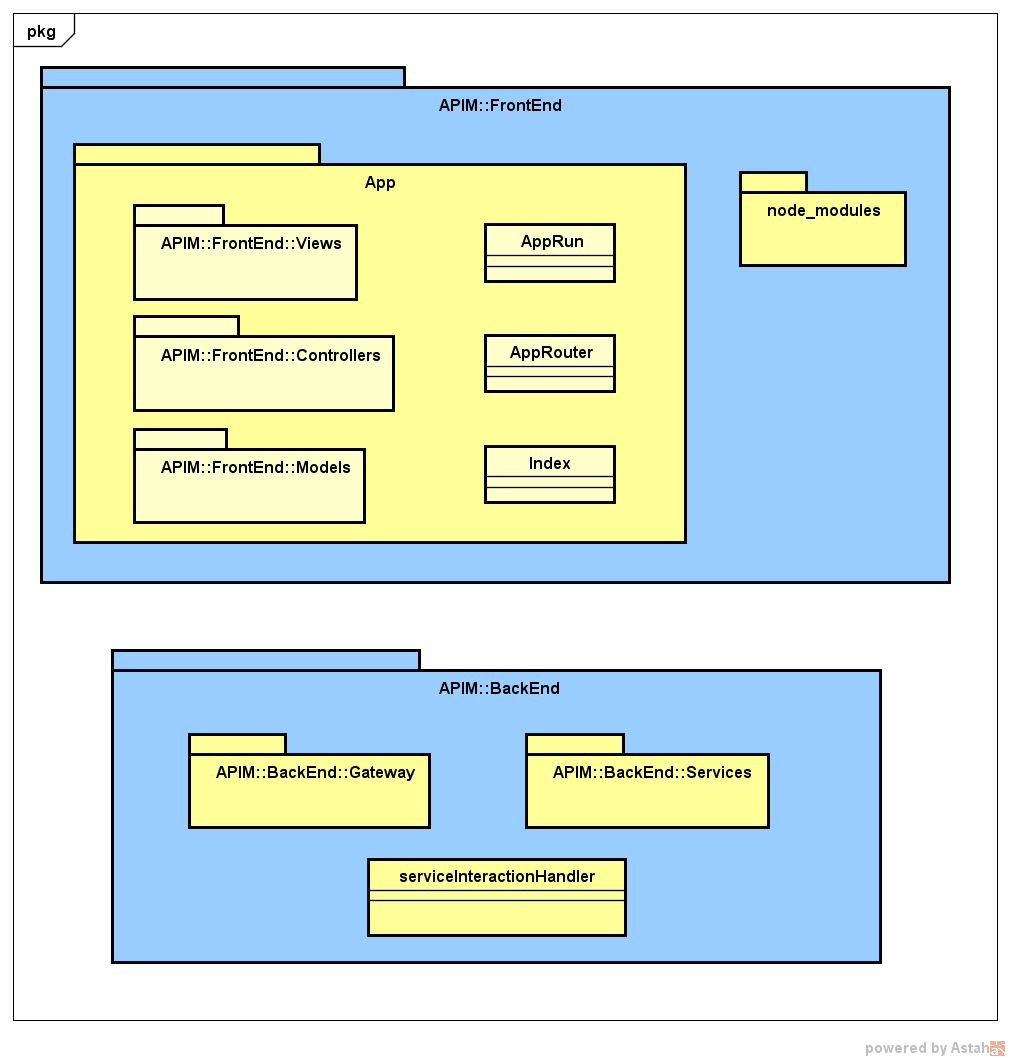
\includegraphics
	[width=0.7\linewidth]
	{images/APIM/Architettura_generale.png}
	\caption{Architettura generale}
\end{figure}

\subsubsection{Informazioni generali}
Di seguito, sono raccolte le informazioni generali dello schema presentato precedentemente:
	\begin{itemize}
		\item \textbf{Descrizione:} architettura ad alto livello della piattaforma \progetto.
		\item \textbf{Packages contenuti:}
		\begin{itemize}
			\item APIM::FrontEnd: package contenente tutti i packages che compongono la parte di front-end dell'applicazione;
			\item APIM::BackEnd: package contenente tutti i packages che compongono la parte di back-end dell'applicazione.
		\end{itemize}
	\end{itemize}

\newpage
\section{Packages Front-end}

\subsection{node\_modules}
\begin{itemize}
	\item \textbf{Padre}: FrontEnd;
	
	\item \textbf{Descrizione}: package che raccoglie le librerie esterne di JavaScript, installate tramite \textit{npm} di Node.js, e fornisce le funzionalità necessarie alla parte di front-end dell'applicazione;
	
	\item \textbf{Relazioni d’uso con altri componenti}: questo package si relaziona con i \textit{controllers} presenti nel sub-package \textit{Controllers} del package \textit{App}.
\end{itemize}

\subsection{App}

\begin{figure}[H]
	\centering
	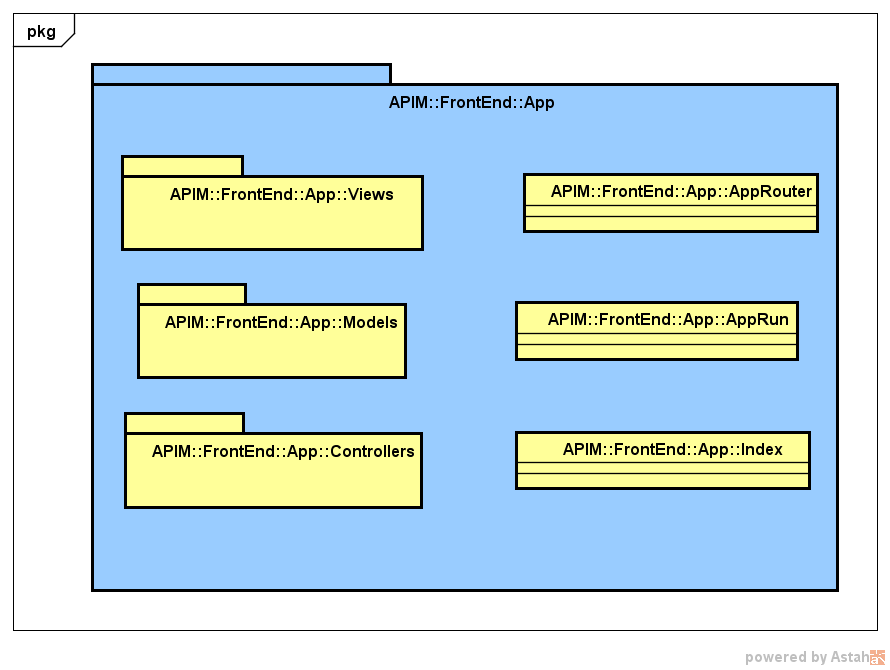
\includegraphics
	[width=0.7\linewidth]
	{UML/DiagrammiPackage/app.png}
	\caption{Package APIM::FrontEnd::App}
\end{figure}

\begin{itemize}
	\item \textbf{Padre}: FrontEnd;
	
	\item \textbf{Descrizione}: package che raccoglie le componenti principali del front-end dell'applicazione web, secondo il pattern architetturale Model-View-Controller (MVC);
	
	\item \textbf{Relazioni d’uso con altri componenti}: questo package si relaziona con le librerie presenti nel sub-package \textit{node\_modules} del package padre;
	
	\item \textbf{Package contenuti}:
	\begin{itemize}
		\item \textbf{\textit{Views}}: package contenente le \textit{views} del front-end dell'applicazione;
		
		\item \textbf{\textit{Models}}: package contenente i \textit{models} del front-end dell'applicazione;
		
		\item \textbf{\textit{Controllers}}: package contenente i \textit{controllers} del front-end dell'applicazione.
	\end{itemize}
	\item \textbf{Classi contenute}:
	\begin{itemize}
		
		\item \textbf{\textit{AppRun}}: classe che istanzia l'applicazione;
		
		\item \textbf{\textit{AppRouter}}: classe che gestisce i routes dell'applicazione;
		
		\item \textbf{\textit{Index}}: view generale dell'applicazione (single page app).
	\end{itemize}
\end{itemize}

\subsubsection{AppRun}

\begin{itemize}
	\item \textbf{Padre}: App;
	
	\item \textbf{Descrizione}: classe che istanzia l'applicazione e che viene utilizzata per indicare le dipendenze tra l'applicazione e i packages esterni.
\end{itemize}

\subsubsection{AppRouter}

\begin{itemize}
	\item \textbf{Padre}: App;
	
	\item \textbf{Descrizione}: classe che gestisce i routes dell'applicazione al fine di associare ad ogni route un controller e una view (associa un URL alle varie view dell'applicazione).
\end{itemize}

\subsubsection{Index}

\begin{itemize}
	\item \textbf{Padre}: App;
	
	\item \textbf{Descrizione}: classe che rappresenta la view generale dell'applicazione e che contiene gli elementi che saranno presenti in ogni pagina dell'applicazione.
\end{itemize}

\subsubsection{Views}

\begin{figure}[H]
	\centering
	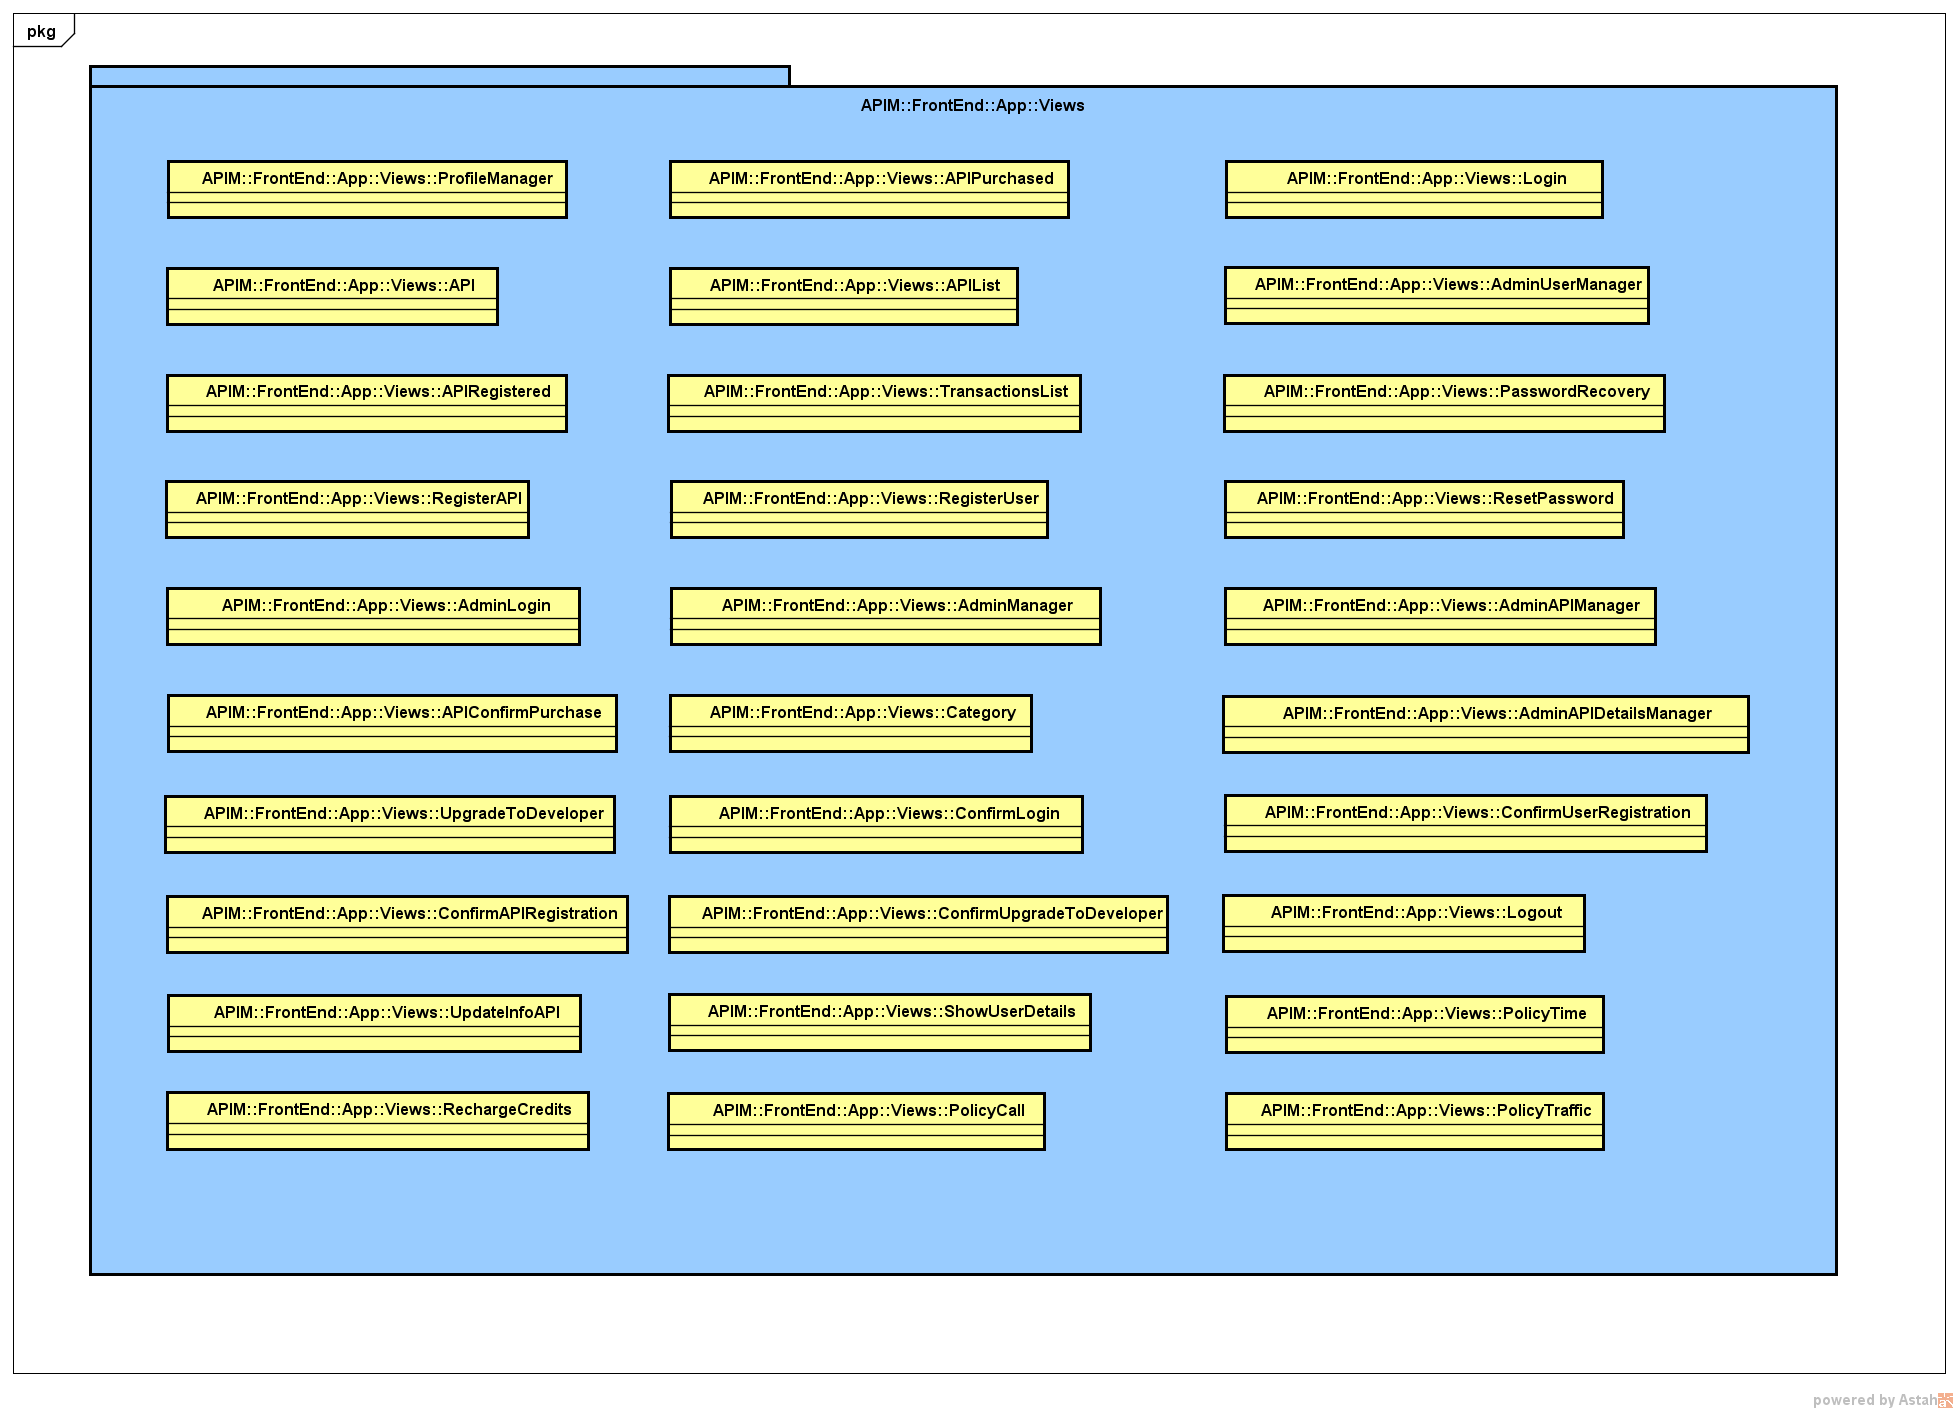
\includegraphics
	[width=0.9\linewidth]
	{UML/DiagrammiPackage/views.png}
	\caption{Package APIM::FrontEnd::App::Views}
\end{figure}

\begin{itemize}
	\item \textbf{Padre}: App;
	
	\item \textbf{Descrizione}: package contenente tutte le classi che rappresentano i vari template HTML per le pagine web dell'applicazione;
	
	\item \textbf{Relazioni d’uso con altri componenti}: questo package si relaziona con i \textit{controllers} presenti nel package \textit{Controllers};
	
	\item \textbf{Classi contenute}:
	\begin{itemize}
		\item \textbf{\textit{RegisterUser}}: view contenente il form dedicato alla registrazione di un utente, il quale può inserire i campi necessari e registrarsi così alla piattaforma. Contiene, inoltre, un link alla pagina di login.\\
		Si relaziona con le seguenti componenti: \textit{UserRegistrationController}.
		
		\item \textbf{\textit{Login}}: view contenente il form necessario affinchè l'utente possa effettuare il login ed autenticarsi al sistema. Contiene, inoltre, un link alla pagina di registrazione e uno alla pagina per il recupero della password.\\
		Si relaziona con le seguenti componenti: \textit{LoginController}.
		
		\item \textbf{\textit{PasswordRecovery}}: view contenente il form dedicato al recupero della password di un utente, il quale può inserire l'indirizzo email e ricevere una nuova password con la quale autenticarsi al sistema. Contiene, inoltre, un link alla pagina di login.\\
		Si relaziona con le seguenti componenti: \textit{PasswordRecoveryController}.
		
		\item \textbf{\textit{API}}: view contenente i risultati della ricerca effettuata, che permette di selezionare un risultato presente al suo interno.\\
		Si relaziona con le seguenti componenti: \textit{APIController}.
		
		\item \textbf{\textit{ProfileManager}}: view contenente le informazioni del profilo personale di un utente registrato. Contiene, inoltre, l'informazione relativa al saldo del proprio conto virtuale.\\
		Si relaziona con le seguenti componenti: \textit{ProfileManagerController}.
		
		\item \textbf{\textit{ResetPassword}}: view contenente il form dedicato al cambio di password di un utente autenticato, il quale può inserire la nuova password che intende utilizzare per i futuri login al sistema.\\
		Si relaziona con le seguenti componenti: \textit{ResetPasswordController}.
		
		\item \textbf{\textit{RegisterAPI}}: view contenente il form per l'inserimento di una API da parte di un utente sviluppatore. Lo sviluppatore può inserire tutti i dati relativi al microservizio che intende esporre sul marketplace.\\
		Si relaziona con le seguenti componenti: \textit{APIRegistrationController}.
		
		\item \textbf{\textit{PolicyCall}}: view contenente le informazioni relative alla policy per chiamate.\\
		Si relaziona con le seguenti componenti: \textit{PolicyCallController}.
		
		\item \textbf{\textit{PolicyTime}}: view contenente le informazioni relative alla policy per tempo.\\
		Si relaziona con le seguenti componenti: \textit{PolicyTimeController}.
		
		\item \textbf{\textit{PolicyTraffic}}: view contenente le informazioni relative alla policy per traffico dati.\\
		Si relaziona con le seguenti componenti: \textit{PolicyTrafficController}.
		
		\item \textbf{\textit{APIRegistered}}: view contenente le informazioni di una API registrata sulla piattaforma.\\
		Si relaziona con le seguenti componenti: \textit{APIRegisteredController}.
		
		\item \textbf{\textit{APIPurchased}}: view contenente le informazioni delle API acquistate da un cliente della piattaforma \progetto.\\
		Si relaziona con le seguenti componenti: \textit{APIPurchasedController}.
		
		\item \textbf{\textit{APIList}}: view contenente l'elenco delle API disponibili sul marketplace \progetto.\\
		Si relaziona con le seguenti componenti: \textit{APIListController}.
		
		\item \textbf{\textit{TransactionsList}}: view contenente l'elenco delle transazioni effettuate da un utente sul marketplace \progetto.\\
		Si relaziona con le seguenti componenti: \textit{TransactionsListController}.
		
		\item \textbf{\textit{APIConfirmPurchase}}: view contenente la conferma di un acquisto di una API.\\
		Si relaziona con le seguenti componenti: \textit{APIConfirmPurchaseController}.
		
		\item \textbf{\textit{AdminManager}}: view contenente le operazioni per la gestione del profilo amministratore \progetto.\\
		Si relaziona con le seguenti componenti: \textit{AdminManagerController}.
		
		\item \textbf{\textit{Category}}: view contenente l'elenco delle categoria nell'\progetto.\\
		Si relaziona con le seguenti componenti: \textit{CategoryController}.
		
		\item \textbf{\textit{ConfirmUpgradeToDeveloper}}: view contenente la conferma dell'upgrade di un utente a sviluppatore nell'\progetto.\\
		Si relaziona con le seguenti componenti: \textit{ConfirmUpgradeToDeveloperController}.
		
		\item \textbf{\textit{ConfirmLogin}}: view contenente la conferma di login all'\progetto.\\
		Si relaziona con le seguenti componenti: \textit{ConfirmLoginController}.
		
		\item \textbf{\textit{ConfirmUserRegistration}}: view contenente la conferma di registrazione all'\progetto.\\
		Si relaziona con le seguenti componenti: \textit{ConfirmUserRegistrationController}.
		
		\item \textbf{\textit{ConfirmAPIRegistration}}: view contenente la conferma di registrazione di una API all'\progetto.\\
		Si relaziona con le seguenti componenti: \textit{ConfirmAPIRegistrationController}.
		
		\item \textbf{\textit{UpgradeToDeveloper}}: view contenente il modulo per diventare sviluppatore all'interno dell'\progetto.\\
		Si relaziona con le seguenti componenti: \textit{UpgradeToDeveloperController}.
		
		\item \textbf{\textit{AdminAPIManager}}: view contenente le operazioni dell'amministratore sulle API dell'\progetto.\\
		Si relaziona con le seguenti componenti: \textit{AdminAPIManagerController}.
		
		\item \textbf{\textit{AdminAPIDetailsManager}}: view contenente le statistiche di una API dell'\progetto.\\
		Si relaziona con le seguenti componenti: \textit{AdminAPIDetailsManagerController}.
		
		\item \textbf{\textit{AdminUserManager}}: view contenente le operazioni di un ammistratore sugli utenti dell'\progetto.\\
		Si relaziona con le seguenti componenti: \textit{AdminUserManagerController}.
		
		\item \textbf{\textit{AdminLogin}}: view contenente il form necessario affinchè l'amministratore possa effettuare il login ed autenticarsi al sistema.\\
		Si relaziona con le seguenti componenti: \textit{AdminLoginController}.
		
		\item \textbf{\textit{Logout}}: view contenente la conferma di logout dall'\progetto.\\
		Si relaziona con le seguenti componenti: \textit{LogoutController}.
		
		\item \textbf{\textit{UpdateInfoAPI}}: view contenente il form dedicato modifica delle informazioni di una API presente nel marketplace \progetto.\\
		Si relaziona con le seguenti componenti: \textit{UpdateInfoAPIController}.
		
		\item \textbf{\textit{RechargeCredits}}: view contenente la possibilità di scegliere quanti crediti ricaricare sul conto personale tra i tagli disponibili.\\
		Si relaziona con le seguenti componenti: \textit{RechargeCreditsController}.
		
		item \textbf{\textit{ShowUserDetalis}}: view contenente le informazioni personali di un utente visualizzabili da altri fruitori del marketplace \progetto.\\
		Si relaziona con le seguenti componenti: \textit{ShowUserDetalisController}.
		
		\item \textbf{\textit{AdminModeration}}: view contenente il form dedicato alla moderazione di un utente o di una API/microservizio da parte di un amministratore della piattaforma \progetto.\\
		Si relaziona con le seguenti componenti: \textit{AdminModerationController}.
	\end{itemize}
\end{itemize}

\subsubsection{Models}

\begin{figure}[H]
	\centering
	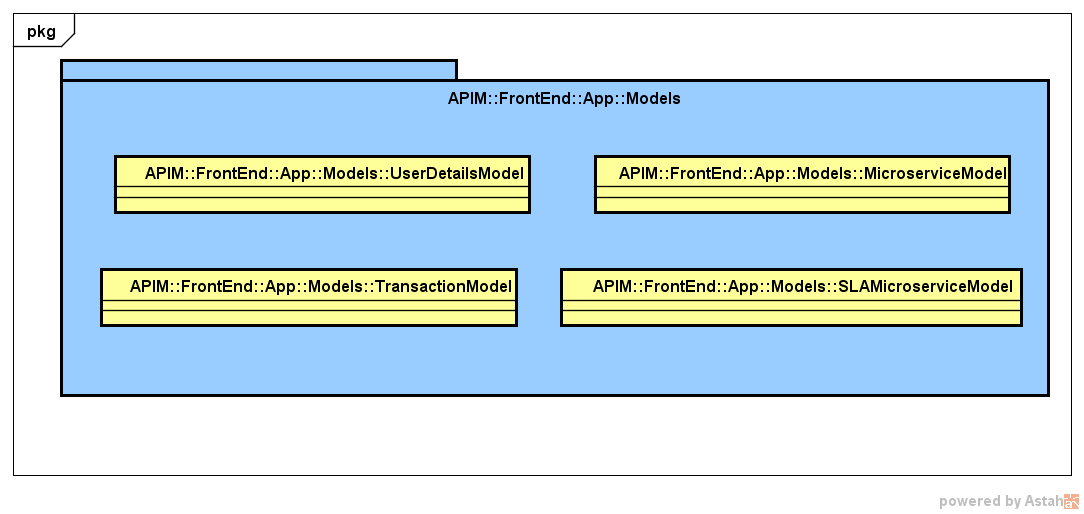
\includegraphics
	[width=0.7\linewidth]
	{UML/DiagrammiPackage/Models.png}
	\caption{Package APIM::FrontEnd::App::Models}
\end{figure}

\begin{itemize}
	\item \textbf{Padre}: App;
	
	\item \textbf{Descrizione}: package che contiene le classi che definiscono la business logic dell'applicazione;
	
	\item \textbf{Relazioni d’uso con altri componenti}: questo package si relaziona con il package \textit{Controllers};
	
	\item \textbf{Classi contenute}:
	\begin{itemize}
		\item \textbf{\textit{UserDetailsModel}}: classe che rappresenta un utente e che contiene tutte le informazioni necessarie alla presentazione del contenuto di un utente, sia nella visualizzazione che nella gestione di un profilo.\\
		Si relaziona con le seguenti componenti: \textit{LoginController}, \textit{APIController}, \textit{ProfileManagerController}, \textit{ResetPasswordController}, \textit{PasswordRecoveryController}.
		
		\item \textbf{\textit{MicroserviceModel}}: classe che rappresenta un microservizio e che contiene tutte le informazioni necessarie alla presentazione del contenuto di un microservizio, sia nella visualizzazione che nella gestione.\\
		Si relaziona con le seguenti componenti: \textit{APIRegiteredController}, \textit{APIRegistrationController}, \textit{PolicyCallController}, \textit{PolicyTimeController}, \textit{PolicyTrafficController}, \textit{APIPurchasedController}, \textit{APIListController}.
		
		\item \textbf{\textit{TransactionModel}}:  classe che rappresenta una transazione avvenuta e che contiene tutte le informazioni necessarie alla presentazione del contenuto di una transazione, sia nella visualizzazione che nella gestione.\\
		Si relaziona con le seguenti componenti: \textit{TransactionsListController}, \textit{APIPurchasedController}.
		
		\item \textbf{\textit{SLAMicroserviceModel}}:  classe che rappresenta la SLA di un microservizio e che contiene tutte le informazioni necessarie alla presentazione del contenuto di SLA di un microservizio, sia nella visualizzazione che nella gestione.\\
		Si relaziona con le seguenti componenti: \textit{PolicyCallController}, \textit{PolicyTimeController}, \textit{PolicyTrafficController}, \textit{APIRegistrationController}.
	\end{itemize}
\end{itemize}

\subsubsection{Controllers}

\begin{figure}[H]
	\centering
	\includegraphics
	[width=0.9\linewidth]
	{UML/DiagrammiPackage/controllers.png}
	\caption{Package APIM::FrontEnd::App::Controllers}
\end{figure}

\begin{itemize}
	\item \textbf{Padre}: App;
	
	\item \textbf{Descrizione}: package che contiene i \textit{controllers} individuati per la parte front-end
	dell'applicazione, i quali consentono la gestione delle azioni utente dell'applicazione web;
	
	\item \textbf{Relazioni d’uso con altri componenti}: questo package si relaziona con i package \textit{Views} e \textit{Models}.
	
	\item \textbf{Classi contenute}:
	\begin{itemize}
		
		\item \textbf{\textit{RegisterUserController}}: classe che permette di gestire la registrazione di un utente al sistema, fornendone le funzionalità preposte.\\
		Si relaziona con le seguenti componenti: \textit{RegisterUser}.
		
		\item \textbf{\textit{LoginController}}: classe che permette di gestire il login di un utente alla piattaforma \progetto, fornendo le funzionalità di autenticazione al sistema, compresa la gestione di	situazioni di errore di autenticazione.\\
		Si relaziona con le seguenti componenti: \textit{UserDetailsModel}, \textit{Login}.
		
		\item \textbf{\textit{PasswordRecoveryController}}: classe che permette di gestire il ripristino della password dimenticata da un utente, fornendo tutte le funzionalità per il recupero della password dopo aver verificato l'identità dell'utente.\\
		Si relaziona con le seguenti componenti: \textit{UserDetailsModel}, \textit{PasswordRecovery}.
		
		\item \textbf{\textit{APIController}}: classe che permette di gestire la ricerca di microservizi all'interno del marketplace \progetto, fornendo all'utente le funzionalità di ricerca tramite categorie e keywords per sviluppatori e microservizi.\\
		Si relaziona con le seguenti componenti: \textit{API}.
		
		\item \textbf{\textit{ProfileManagerController}}: classe che permette di gestire il profilo personale di un utente, fornendo le funzionalità all'utente per poter modificare i propri dati.\\
		Si relaziona con le seguenti componenti: \textit{UserDetailsModel}, \textit{ProfileManager}.
		
		\item \textbf{\textit{ResetPasswordController}}: classe che permette di gestire il cambio password di un utente autenticato al sistema, fornendo le funzionalità per il salvataggio di una nuova password.\\
		Si relaziona con le seguenti componenti: \textit{UserDetailsModel}, \textit{ResetPassword}.
		
		\item \textbf{\textit{RegisterAPIController}}: classe che permette di gestire l'inserimento di una API, fornendo tutte le funzionalità atte alla corretta esposizione di un microservizio di uno sviluppatore, utente della piattaforma \progetto.\\
		Si relaziona con le seguenti componenti: \textit{MicroserviceModel}, \textit{RegisterAPI}.
		
		\item \textbf{\textit{PolicyCallController}}: classe che permette di gestire le policy di vendita dei microservizi per chiamate.\\
		Si relaziona con le seguenti componenti: \textit{PolicyCall}, \textit{SLAMicroserviceModel}.
		
		\item \textbf{\textit{PolicyTimeController}}: classe che permette di gestire le policy di vendita dei microservizi per tempo.\\
		Si relaziona con le seguenti componenti: \textit{PolicyTime}, \textit{SLAMicroserviceModel}.
		
		\item \textbf{\textit{PolicyTrafficController}}: classe che permette di gestire le policy di vendita dei microservizi per traffico dati.\\
		Si relaziona con le seguenti componenti: \textit{PolicyTraffic}, \textit{SLAMicroserviceModel}.
		
		\item \textbf{\textit{APIRegisteredController}}: classe che permette di gestire le informazioni di una API precedentemente inserita.\\
		Si relaziona con le seguenti componenti: \textit{MicroserviceModel}, \textit{APIRegistered}.
		
		\item \textbf{\textit{APIPurchasedController}}: classe che permette di gestire l'acquisto e le relative informazioni di una API, fornendo l'API Key per l'utilizzo del cliente.\\
		Si relaziona con le seguenti componenti: \textit{APIPurchased}, \textit{MicroserviceModel}, \textit{TransactionModel}.
		
		\item \textbf{\textit{APIListController}}: classe che permette di gestire l'elenco dei microservizi presenti sul marketplace \progetto.\\
		Si relaziona con le seguenti componenti: \textit{APIList}, \textit{MicroserviceModel}.
		
		\item \textbf{\textit{TransactionsListController}}: classe che permette di gestire lo storico delle transazioni di un utente del marketplace \progetto.\\
		Si relaziona con le seguenti componenti: \textit{TransactionsList}, \textit{TransactionsModel}.
		
		\item \textbf{\textit{AdminManagerController}}: classe che permette di gestire il profilo di un amministratore della piattaforma \progetto, fornendo le funzionalità per poter modificare i propri dati e moderare utenti ed API.\\
		Si relaziona con le seguenti componenti: \textit{AdminManager}.
		%----------------------
		
		\item \textbf{\textit{CategoryController}}: classe che permette di gestire l'elenco delle categoria nell'\progetto.\\
		Si relaziona con le seguenti componenti: \textit{Category}.
		
		\item \textbf{\textit{ConfirmUpgradeToDeveloperController}}: classe che permette di gestire la conferma dell'upgrade di un utente a sviluppatore nell'\progetto.\\
		Si relaziona con le seguenti componenti: \textit{ConfirmUpgradeToDeveloper}.
		
		\item \textbf{\textit{ConfirmLoginController}}: classe che permette di gestire la conferma di login all'\progetto.\\
		Si relaziona con le seguenti componenti: \textit{ConfirmLogin}.
		
		\item \textbf{\textit{ConfirmUserRegistrationController}}: classe che permette di gestire la conferma di registrazione all'\progetto.\\
		Si relaziona con le seguenti componenti: \textit{ConfirmUserRegistration}.
		
		\item \textbf{\textit{ConfirmAPIRegistrationController}}: classe che permette di gestire la conferma di registrazione di una API all'\progetto.\\
		Si relaziona con le seguenti componenti: \textit{ConfirmAPIRegistration}.
		
		\item \textbf{\textit{UpgradeToDeveloperController}}: classe che permette di gestire il modulo per diventare sviluppatore all'interno dell'\progetto.\\
		Si relaziona con le seguenti componenti: \textit{UpgradeToDeveloper}.
		
		\item \textbf{\textit{AdminAPIManagerController}}: classe che permette di gestire le operazioni dell'amministratore sulle API dell'\progetto.\\
		Si relaziona con le seguenti componenti: \textit{AdminAPIManager}.
		
		\item \textbf{\textit{AdminAPIDetailsManagerController}}: classe che permette di gestire le statistiche di una API dell'\progetto.\\
		Si relaziona con le seguenti componenti: \textit{AdminAPIDetailsManager}.
		
		\item \textbf{\textit{AdminUserManagerController}}: classe che permette di gestire le operazioni di un ammistratore sugli utenti dell'\progetto.\\
		Si relaziona con le seguenti componenti: \textit{AdminUserManager}.
		
		\item \textbf{\textit{AdminLoginController}}: classe che permette di gestire il form necessario affinchè l'amministratore possa effettuare il login ed autenticarsi al sistema.\\
		Si relaziona con le seguenti componenti: \textit{AdminLogin}.
		
		\item \textbf{\textit{LogoutController}}: classe che permette di gestire la conferma di logout dall'\progetto.\\
		Si relaziona con le seguenti componenti: \textit{Logout}.
		
		\item \textbf{\textit{UpdateInfoAPIController}}: classe che permette di gestire il form dedicato modifica delle informazioni di una API presente nel marketplace \progetto.\\
		Si relaziona con le seguenti componenti: \textit{UpdateInfoAPI}.
		
		\item \textbf{\textit{RechargeCreditsController}}: classe che permette di gestire la possibilità di scegliere quanti crediti ricaricare sul conto personale tra i tagli disponibili.\\
		Si relaziona con le seguenti componenti: \textit{RechargeCredits}.
		
		\item \textbf{\textit{ShowUserDetalisController}}: classe che permette di gestire le informazioni personali di un utente visualizzabili da altri fruitori del marketplace \progetto.\\
		Si relaziona con le seguenti componenti: \textit{ShowUserDetalis}
		
		
		%---------------------
		
		\item \textbf{\textit{AdminModerationController}}: classe che permette di gestire la moderazione di un utente (cliente o sviluppatore che sia) e di API, fornendo le funzionalità per la sospensione e rimozione.\\
		Si relaziona con le seguenti componenti: \textit{AdminModeration}.
		
	\end{itemize}
\end{itemize}
\newpage
\subsection{Back-end}

Nella parte back-end sono presenti i package \textit{Gateway} e \textit{Services} strutturati secondo un'architettura a microservizi, i quali hanno una dipendenza verso l'interfaccia \textit{serviceInteractionHandler}.

\begin{figure}[H]
	\centering
	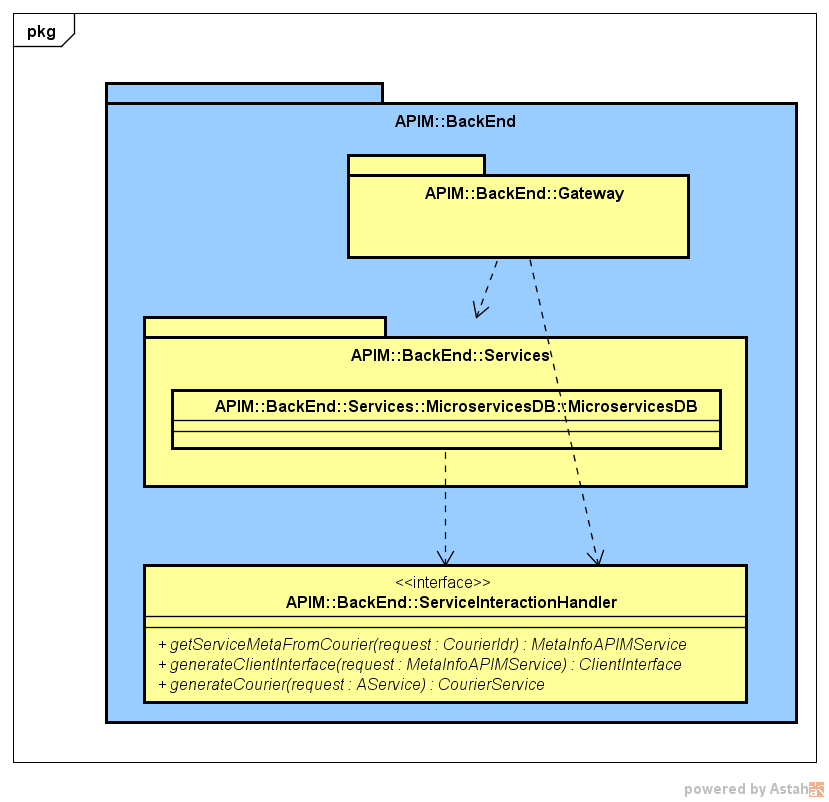
\includegraphics
	[width=0.7\linewidth]
	{UML/DiagrammiPackage/BackEnd.png}
	\caption{Package APIM::BackEnd}
\end{figure}

\begin{itemize}
	\item \textbf{Padre}: APIM;
	
	\item \textbf{Descrizione}: package contenente le componenti del back-end dell'applicazione;
	
	\item \textbf{Package contenuti}:
	\begin{itemize}
		\item \textbf{\textit{Gateway}}: package contenente le classi e le interfacce per il funzionamento dell'API Gateway;
		
		\item \textbf{\textit{Services}}: package contenente tutti i microservizi per le comunicazioni con i database.
	\end{itemize}
	\item \textbf{Classi contenute}:
		\begin{itemize}
			\item \textbf{\textit{serviceInteractionHandler}}: interfaccia per la gestione delle comunicazioni dell'API Gateway e dei \textit{services}.
		\end{itemize}
\end{itemize}

\subsubsection{Gateway}
\begin{figure}[H]
	\centering
	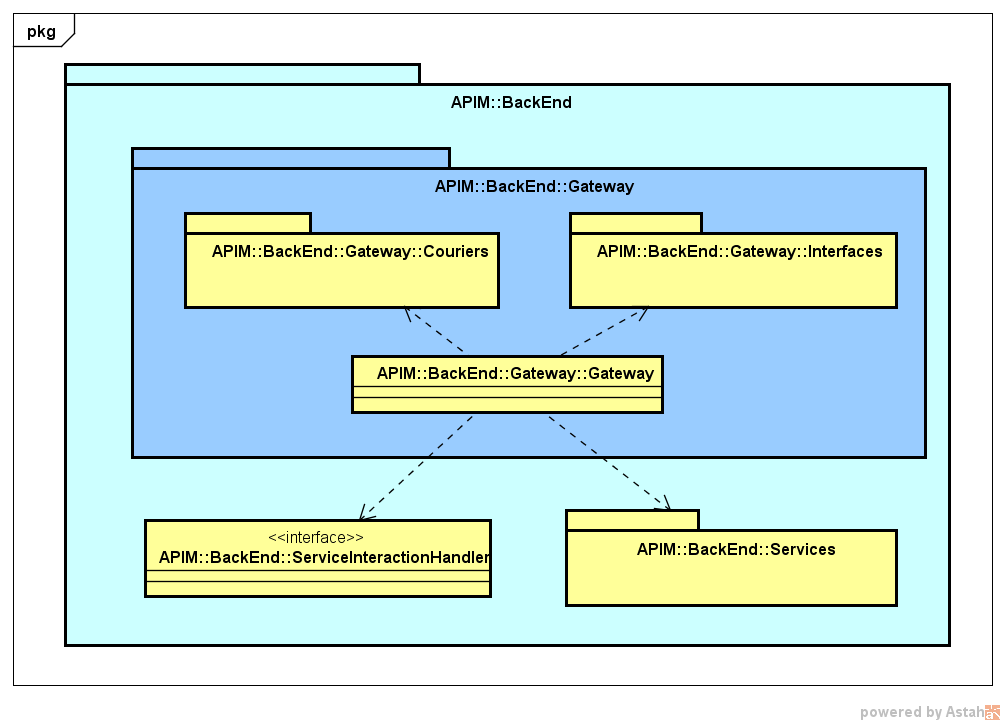
\includegraphics
	[width=0.7\linewidth]
	{UML/DiagrammiPackage/gateway.png}
	\caption{Package APIM::BackEnd::Gateway}
\end{figure}

\begin{itemize}
	\item \textbf{Padre}: BackEnd;
	
	\item \textbf{Descrizione}: package contenente la componente principale del lato back-end. Pur essendo integrato nella sistema, è un modulo che svolge funzioni separate alla piattaforma vera e propria: infatti, l'API Gateway si occupa di controllare e reindirizzare le chiamate effettuate dai clienti ai microservizi (prodotti) inseriti nel marketplace \progetto, verificandone la validità (credenziali, chiave) e monitorandone l'uso (SLA, utilizzi rimanenti).
	
	\item \textbf{Relazioni d'uso con altri componenti}: la classe \textit{Gateway} comunica con le classi contenute all'interno del package \textit{Services}. Inoltre, necessita delle interfacce contenute nel package \textit{Interfaces} e crea le sessioni \textit{couriers} Jolie, archiviandole nel package \textit{Couriers}.
	
	\item \textbf{Package contenuti}:
	\begin{itemize}
		\item \textbf{\textit{Couriers}}: package contenente l'archivio delle sessioni couriers dei microservizi Jolie. Le sessioni couriers vengono create dal gateway ed utilizzate da \textit{serviceinteractionhandler}. Inoltr, forniscono i dati necessari al funzionamento del package \textit{Interfaces}.\\
		Le sessioni couriers permettono l'overloading dei messaggi inviati nelle chiamate dei microservizi al gateway, così da allegare alla richiesta le informazioni per raggiungere il microservizio desiderato.
		
		\item \textbf{\textit{Interfaces}}: package contenente le interfacce necessarie al funzionamento dell'API Gateway. Si occupa dei dati riguardanti le chiamate ai microservizi, in particolar modo, il tipo di operazione richiesta e le informazioni riguardanti l'interfaccia del microservizio target.
	\end{itemize}
	\item \textbf{Classi contenute}:
		\begin{itemize}
			\item \textbf{\textit{Gateway}}: classe che rappresenta la struttura dell'API Gateway della piattaforma \progetto.
		\end{itemize}
\end{itemize}

\subsubsection{Services}
Tale package contiene tutti i servizi appartenenti al lato back-end della piattaforma, eccezion fatta per il gateway già descritto nella sezione soprastante. \textit{Services} contiene tutte le classi di comunicazione con i database che permetteranno il corretto funzionamento dell'applicazione.

\begin{figure}[H]
	\centering
	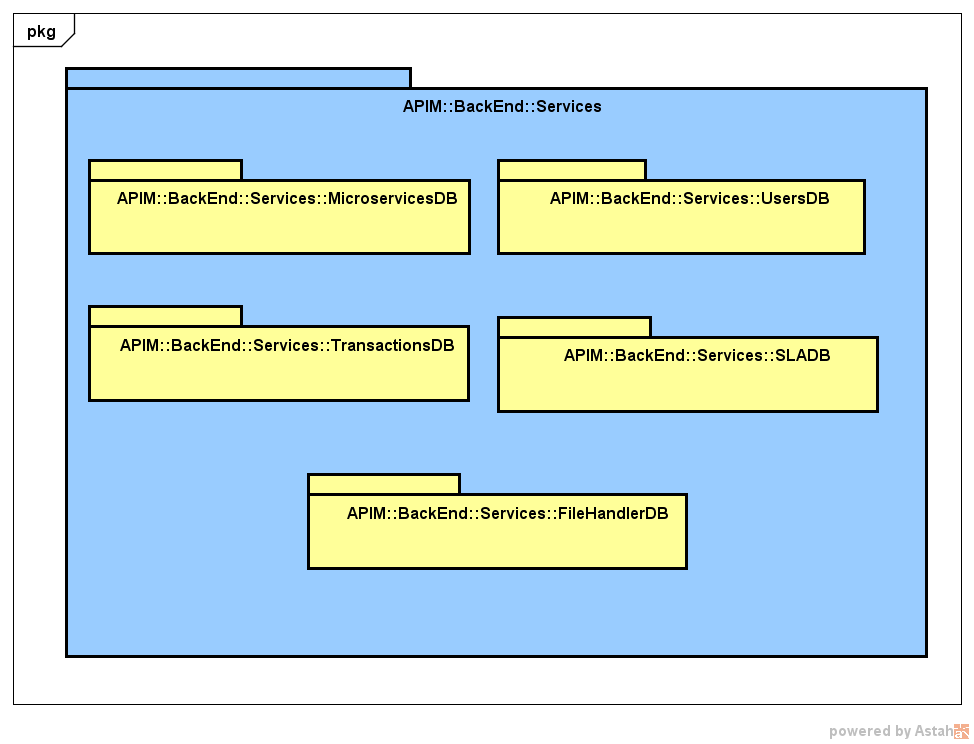
\includegraphics
	[width=0.7\linewidth]
	{UML/DiagrammiPackage/services.png}
	\caption{Package APIM::BackEnd::Services}
\end{figure}

\begin{itemize}
	\item \textbf{Padre}: BackEnd;
	
	\item \textbf{Descrizione}: package che contiene tutti i package relativi ai microservizi del back-end dell'applicazione;
	
	\item \textbf{Relazioni d'uso con altri componenti}: questo package si relaziona con l'API Gateway;
	
	\item \textbf{Package contenuti}:
	\begin{itemize}
		\item \textbf{\textit{UsersDB}}: package contenente le classi che permettono la comunicazione con il database relativo agli utenti del sistema;
		
		\item \textbf{\textit{MicroservicesDB}}: package contenente le classi che permettono la comunicazione con il database relativo ai microservizi registrati sulla piattaforma;
		
		\item \textbf{\textit{TransactionsDB}}: package contenente le classi che permettono la comunicazione con il database relativo alle transazioni degli utenti del sistema;
		
		\item \textbf{\textit{SLADB}}: package contenente le classi che permettono la comunicazione con il database relativo alle informazioni di SLA dei microservizi utilizzati tramite l'API Gateway della piattaforma \progetto;
		
		\item \textbf{\textit{FileHandlerDB}}: package contenente le classi che permettono la gestione dei file;
		
		\item \textbf{\textit{FrontEndMS}}: package contenente le classi che si occupano delle operazioni più complesse, quali l'accesso a più di un database.
	\end{itemize}
\end{itemize}

\paragraph{UsersDB}

\begin{figure}[H]
	\centering
	\includegraphics
	[width=0.7\linewidth]
	{UML/DiagrammiPackage/Users_db.png}
	\caption{Package APIM::BackEnd::Services::UsersDB}
\end{figure}

\begin{itemize}
	\item \textbf{Padre}: Services;
	
	\item \textbf{Descrizione}: package che contiene le classi di comunicazione con il database dell'applicazione relativo alle informazioni (anagrafiche e personali) degli utenti (admin, clienti, sviluppatori) del sistema;
	
	\item \textbf{Relazioni d'uso con altri componenti}: questo package si relaziona con il sub-package \textit{FrontEndMS} del package padre, fornendogli i dati che esso richiede riguardo alle operazioni con il database delle informazioni degli utenti;
	
	\item \textbf{Classi contenute}:
		\begin{itemize}
			\item \textbf{\textit{Users\_dbInterface}}: interfaccia che raccoglie tutte le \textit{operation} riguardanti il database degli utenti;
			
			\item \textbf{\textit{Users\_db}}: classe che implementa l'interfaccia \textit{Users\_dbInterface}.
		\end{itemize}
\end{itemize}

\paragraph{MicroservicesDB}

\begin{figure}[H]
	\centering
	\includegraphics
	[width=0.7\linewidth]
	{UML/DiagrammiPackage/MicroservicesDB.png}
	\caption{Package APIM::BackEnd::Services::MicroservicesDB}
\end{figure}

\begin{itemize}
	\item \textbf{Padre}: Services;
	
	\item \textbf{Descrizione}: package che contiene le classi di comunicazione con il database dell'applicazione relativo ai microservizi registrati nella piattaforma;
	
	\item \textbf{Relazioni d'uso con altri componenti}: questo package si relaziona con il package \textit{FrontendMS}, fornendogli i dati che esso richiede riguardo alle operazioni con il database delle informazioni dei microservizi.\\
	Inoltre, comunica con il Gateway per permettere l'identificazione e l'utilizzo dei microservizi, e garantire correttezza, efficienza e validità delle chiamate;
	
	\item \textbf{Classi contenute}:
	\begin{itemize}
		\item \textbf{\textit{Microservices\_dbInterface}}: interfaccia che raccoglie tutte le \textit{operation} riguardanti il database dei microservizi;
		
		\item \textbf{\textit{Microservices\_db}}: classe che implementa le interfacce \textit{Microservices\_dbInterface} e \textit{serviceInteractionHandler}.
	\end{itemize}
\end{itemize}

\paragraph{TransactionsDB}

\begin{figure}[H]
	\centering
	\includegraphics
	[width=0.7\linewidth]
	{UML/DiagrammiPackage/Transactions_db.png}
	\caption{Package APIM::BackEnd::Services::TransactionsDB}
\end{figure}

\begin{itemize}
	\item \textbf{Padre}: Services;
	
	\item \textbf{Descrizione}: package che contiene le classi di comunicazione con il database dell'applicazione che si occupa di immagazzinare i dati sulle transazioni;
	
	\item \textbf{Relazioni d'uso con altri componenti}: questo package si relaziona con il package \textit{FrontendMS}, fornendogli i dati che esso richiede riguardo alle operazioni con il database delle informazioni delle transazioni.\\
	Comunica inoltre con il Gateway per verificare la validità delle API Key e/o aggiornare i dati relativi (usi residui della chiave) alle chiamate ai microservizi effettuate;
	
	\item \textbf{Classi contenute}:
	\begin{itemize}
		\item \textbf{\textit{Transactions\_dbInterface}}: interfaccia che raccoglie tutte le \textit{operation} riguardanti il database delle transazioni;
		
		\item \textbf{\textit{Transactions\_db}}: classe che implementa l'interfaccia \textit{Transactions\_dbInterface}.
	\end{itemize}
\end{itemize}

\paragraph{SLADB}

\begin{figure}[H]
	\centering
	\includegraphics
	[width=0.7\linewidth]
	{UML/DiagrammiPackage/SLA_db.png}
	\caption{Package APIM::BackEnd::Services::SLADB}
\end{figure}

\begin{itemize}
	\item \textbf{Padre}: Services;
	
	\item \textbf{Descrizione}: package che contiene le classi di comunicazione con il database che si occupa di immagazzinare e trattare i dati relativi al Service Level Agreement (SLA);
	
	\item \textbf{Relazioni d'uso con altri componenti}: questo package si relaziona con il package \textit{FrontendMS}, fornendogli i dati che esso richiede riguardo alle operazioni con il database delle informazioni della SLA.\\
	Inoltre, comunica con il Gateway per aggiornare i dati delle performance di risposta di ogni microservizio utilizzato;
	
	\item \textbf{Classi contenute}:
	\begin{itemize}
		\item \textbf{\textit{SLA\_dbInterface}}: interfaccia che raccoglie tutte le \textit{operation} riguardanti il database delle informazioni di SLA;
		
		\item \textbf{\textit{SLA\_db}}: classe che implementa l'interfaccia \textit{SLA\_dbInterface}.
	\end{itemize}
\end{itemize}

\paragraph{FileHandlerDB}

\begin{figure}[H]
	\centering
	\includegraphics
	[width=0.7\linewidth]
	{UML/DiagrammiPackage/FileHandlerDB.png}
	\caption{Package APIM::BackEnd::Services::FileHandlerDB}
\end{figure}

\begin{itemize}
	\item \textbf{Padre}: Services;
	
	\item \textbf{Descrizione}: package che si occupa della gestione dei file, e presenta le classi di comunicazione con il database per tale finalità;
	
	\item \textbf{Relazioni d'uso con altri componenti}: questo package si relaziona con il package \textit{FrontendMS}, fornendogli i dati che esso richiede riguardo alle operazioni con il database delle informazioni dei file.\\
	Inoltre, comunica con il Gateway per recuperare i file legati alle interfacce dei microservizi;
	
	\item \textbf{Classi contenute}:
	\begin{itemize}
		\item \textbf{\textit{FileHandlerInterface}}: interfaccia che raccoglie tutte le \textit{operation} riguardanti la gestione dei file;
		
		\item \textbf{\textit{FileHandler}}: classe che implementa l'interfaccia \textit{FileHandlerInterface}.
	\end{itemize}
\end{itemize}

\paragraph{FrontendMS}

\begin{figure}[H]
	\centering
	\includegraphics
	[width=0.7\linewidth]
	{UML/DiagrammiPackage/FrontEndMS.png}
	\caption{Package APIM::BackEnd::Services::FrontEndMS}
\end{figure}

\begin{itemize}
	\item \textbf{Padre}: Services;
	
	\item \textbf{Descrizione}: package che si occupa delle operazioni più complesse, che accedono a più database e devono rielaborarne i dati. La maggior parte delle funzionalità garantite dal front-end passano per questo servizio, in quanto occorre raccogliere dati da più database e/o raffinare le informazioni grezze dei \textit{services};
	
	\item \textbf{Relazioni d'uso con altri componenti}: questo package si relaziona con tutti gli altri package e relativi servizi del package padre, quali \textit{UsersDB}, \textit{MicroservicesDB}, \textit{TransactionsDB}, \textit{SLADB} e \textit{FileHandlerDB};
	
	\item \textbf{Classi contenute}:
	\begin{itemize}
		\item \textbf{\textit{FrontEndInterface}}: interfaccia che raccoglie tutte le \textit{operation} più complesse, come ad esempio la gestione della visualizzazione della home del marketplace;
		
		\item \textbf{\textit{FrontEndMS}}: classe che implementa l'interfaccia \textit{FrontEndInterface}.
	\end{itemize}
\end{itemize}

%\newpage
\section{Amministrazione di sistema}

\subsection{Dati superuser}

\subsection{Descrizione}

\subsection{Operazioni disponibili}


\newpage
\section{Implementazione funzionalità}

\subsection{Front-end}

\subsection{Back-end}

\appendix
\newpage
\section{Glossario}

%\hypertarget{A}{}

\newglossaryentry{AlexaSDK}
{
	name=AlexaSDK,
	description={sistema di comando vocale sviluppato da Amazon}
}
\newglossaryentry{Android}
{
	name=Android,
	description={sistema operativo open source per dispositivi mobili, sviluppato da Google Inc. e basato su kernel Linux. Inoltre, mette a disposizione una piattaforma per lo sviluppo di applicazioni per dispositivi mobili}
}
\newglossaryentry{Angular2}
{
	name=Angular 2,
	description={framework gratuito per il front-end web, open source ed evoluzione di AngularJS. \MakeUppercase{è} scritto in linguaggio TypeScript}
}
\newglossaryentry{API}
{
	name=API,
	description={acronimo per Application Programming Interface, indica un insieme di funzioni software ad alto livello disponibili al programmatore. Solitamente sono composte di poche istruzioni volte alla realizzazione di una specifica azione. Un esempio di API sono le librerie software messe a disposizione da un certo linguaggio di programmazione}
}
\newglossaryentry{API Gateway}
{
	name=API Gateway,
	description={strumento che filtra e reindirizza le richieste utente per le varie API, fornendo il servizio, anche se questo non è presente sul server del marketplace}
}
\newglossaryentry{API Key}
{
	name=API Key,
	description={codice che identifica univocamente una specifica API e funge da token segreto che ne regola l'accesso e l'utilizzo}
}
\newglossaryentry{API Market}
{
	name=API Market,
	description={piattaforma che permette il commercio di API}
}
\newglossaryentry{Asana}
{
	name=Asana,
	description={applicazione web, disponibile anche per dispositivi mobili, progettata per aiutare i team di progetto a monitorare il proprio lavoro e migliorare la collaborazione. Ogni progetto è composto di più attività, chiamate task, le quali richiedono lo svolgimento di determinati compiti. Gli utenti possono aggiungere note, commenti, allegati e tag, il tutto notificando, via email automatica o notifica push, ogni altro membro del team che lavora al progetto}
}
\newglossaryentry{Astah}
{
	name=Astah,
	description={strumento di modellazione UML per la creazione di vari tipi di diagrammi. La versione Community è gratuita, a differenza di quella Professional}
}
\newglossaryentry{AWS}
{
	name=AWS,
	description={acronimo per Amazon Web Services, rappresenta una collezione di servizi di cloud computing che compongono la piattaforma on demand (su richiesta) offerta dall'azienda Amazon. Questi servizi sono operativi in 12 regioni geografiche in cui Amazon stessa ha suddiviso il globo. Tra questi servizi i più conosciuti sono Amazon Elastic Compute Cloud (EC2) e Amazon Simple Storage Service (S3)}
}
\newglossaryentry{AWS Lambda}
{
	name=AWS Lambda,
	description={servizio di elaborazione serverless, che esegue il codice utente in risposta a determinati eventi e gestisce automaticamente le risorse di elaborazione, tra cui la manutenzione di server e del sistema operativo, il provisioning e il ridimensionamento automatico della capacità, lo sviluppo di patch per codice e protezione e il monitoraggio e la creazione di log. Può essere usato per estendere altri servizi AWS con logica personalizzata oppure creare servizi di back-end in grado di operare con la scalabilità, le prestazioni e la sicurezza di AWS}
}


%\newpage
%\hypertarget{B}{}

\newglossaryentry{back-end}
{
	name=back-end,
	description={Parte di un sistema informatico che elabora i dati generati dal front-end}
}

\newglossaryentry{Bootstrap 3}
{
	name=Bootstrap 3,
	description={Framework gratuito per il front-end web, open source, per la progettazione di siti e applicazioni web. Contiene template CSS per la maggior parte delle componenti grafiche di un'interfaccia utente ed estensioni JavaScript. A differenza di molti altri framework web, Bootstrap si occupa solo della parte front-end}
}

\newglossaryentry{browser}
{
	name=browser,
	description={Applicazione per il recupero, la presentazione e la navigazione di risorse sul web}
}
%\newpage
%\hypertarget{C}{}

\newglossaryentry{Camel Case}
{
	name=Camel Case,
	description={La Notazione a Cammello o in inglese Camel Case è la pratica nata durante gli anni settanta di scrivere parole composte o frasi unendo tutte le parole tra loro, ma lasciando le loro iniziali maiuscole}
}

\newglossaryentry{client}
{
	name=client,
	description={componente che accede ai servizi o alle risorse messe a disposizione da un server. Esso fa parte dell'architettura logica di rete client-server. Inoltre, il termine client indica anche il software usato sul computer-client per accedere alle funzionalità offerte da un server}
}

\newglossaryentry{cloud computing}
{
	name=cloud computing,
	description={letteralmente "nuvola informatica", indica un paradigma di erogazione di risorse informatiche come l'archiviazione, l'elaborazione o la trasmissione di dati, caratterizzato dalla disponibilità on demand attraverso Internet, a partire da un insieme di risorse preesistenti e configurabili}
}

\newglossaryentry{CSS}
{
	name=CSS,
	description={acronimo per Cascading Style Sheets (letteralmente fogli di stile a cascata), è un linguaggio usato per definire la formattazione di documenti HTML, XHTML e XML}
}

\newglossaryentry{CSS3}
{
	name=CSS3,
	description={ultima versione dello standard CSS. \MakeUppercase{è} retrocompatibile con le precedenti versioni di CSS}
}

\newglossaryentry{CSSLint}
{
	name=CSSLint,
	description={strumento che aiuta a rilevare possibili errori nel codice CSS}
}

\newglossaryentry{customer communication dashboard}
{
	name=customer communication dashboard,
	description={interfaccia grafica che organizza e presenta le informazioni circa l'acquisto o la disdetta di API in modo semplice, intuitivo ed immediato, consentendo al management di agire tempestivamente nella correzione della strategia in caso di necessità}
}



	

%\newpage
%\newpage
\section{D}

\begin{itemize}
	\item \textbf{Database NoSQL}: si differenziano dai database SQL per il fatto che i dati vengono conservati in documenti e non in tabelle. Le informazioni non sono distribuite in differenti strutture logiche, ma vengono aggregate per oggetto in documenti, la cui natura può essere di tipo Key-Value (che rappresenta la forma primitiva di database NoSQL) o Document Store, basati su semantica JSON. Ogni documento aggregato raccoglie tutti i dati associati a un’entità, in modo che qualsiasi applicazione possa trattare l’entità come oggetto e valutare in un sol colpo tutte le informazioni a essa correlate. In questo modo, si evitano anche i fardelli computazionali dovuti ai passaggi di aggregazione delle informazioni tipici del linguaggio SQL, in quanto tutti i dati necessari e corrispondenti a un medesimo oggetto sono già disponibili in un unico documento. L’assenza di tabelle permette ai database non relazionali di essere schemaless, ossia privi di un qualsiasi schema definito a priori, e questa caratteristica conferisce ai database NoSQL un altro vantaggio non trascurabile.
	\item \textbf{Database SQL}: sono basati sul modello relazionale (RDBMS) progettato per:
	\begin{enumerate}  
		\item Creare e modificare schemi di database (DDL - Data Definition Language);
		\item Inserire, modificare e gestire dati memorizzati (DML - Data Manipulation Language);
		\item Creare e gestire strumenti di controllo ed accesso ai dati (DCL - Data Control Language).
	\end{enumerate}
	\item \textbf{Diagramma dei package}: in UML, i packages vengono usati per raggruppare elementi e fornire un namespace per gli elementi raggruppati. Un package può contenere altri packages o altri elementi UML (ad esempio, classi, oggetti, casi d'uso, componenti, nodi, istanze di nodi, etc.), consentendo un'organizzazione gerarchica dei vari elementi che descrivono un sistema.
	\item \textbf{Diagramma delle classi}: tipo di diagramma che può comparire in un modello UML, il quale consente di descrivere tipi di entità, con le loro caratteristiche e le eventuali relazioni fra questi tipi. Gli strumenti concettuali utilizzati sono il concetto di classe del paradigma object-oriented e altri correlati, per esempio la generalizzazione, che è una relazione concettuale assimilabile al meccanismo object-oriented dell'ereditarietà
	\item \textbf{Diagramma di attività}: diagramma definito all'interno dello Unified Modeling Language (UML), che definisce le attività da svolgere per realizzare una data funzionalità. Può essere utilizzato durante la progettazione del software, per dettagliare un determinato algoritmo. In particolare, definisce le relazioni tra le attività, i responsabili per le singole attività e i punti di decisione. \MakeUppercase{è} spesso usato come modello complementare ai diagrammi dei casi d'uso, per descrivere le dinamiche con cui si sviluppano
	\item \textbf{Diagramma di Gantt}: è usato principalmente nelle attività di project management, ed è costruito partendo da un asse orizzontale, a rappresentazione dell'arco temporale totale del progetto, suddiviso in fasi incrementali, e da un asse verticale, a rappresentazione delle mansioni o attività che costituiscono il progetto. Un diagramma di Gantt permette la rappresentazione grafica di un calendario di attività, utile al fine di pianificare, coordinare e tracciare specifiche attività in un progetto, dando una chiara illustrazione dello stato d'avanzamento del progetto rappresentato.
	\item \textbf{Diagramma di sequenza}: diagramma previsto dallo standard UML, utilizzato per descrivere uno scenario, ovvero una sequenza di azioni in cui tutte le scelte sono state già effettuate. Descrive le relazioni che intercorrono, in termini di messaggi, tra attori, oggetti di business, oggetti o entità del sistema che si sta rappresentando
	\item \textbf{Django}: web framework open source per lo sviluppo di applicazioni web, scritto in linguaggio Python, seguendo il design pattern MVC (Model-View-Controller)
	\item \textbf{DynamoDB}: servizio di database NoSQL completamente gestito e messo a disposizione da Amazon. Esso consente di scaricare gli oneri amministrativi di funzionamento e di scalare un database distribuito, in modo che l'utente non debba preoccuparsi di nulla.
	Con DynamoDB, è possibile creare le tabelle del database in grado di memorizzare e recuperare qualsiasi quantità di dati, servire qualsiasi livello di richiesta di traffico, e utilizzare la console di gestione AWS per monitorare le metriche di utilizzo delle risorse e di prestazioni. Infine, diffonde automaticamente i dati e il traffico per le tabelle su di un numero sufficiente di server per gestire le esigenze dell'utente, mantenendo prestazioni costanti e veloci. Tutti i dati sono memorizzati su dischi SSD e replicati automaticamente su più Availability Zones (zone di disponibilità) in una regione AWS.
\end{itemize}



%\newpage
%\newpage
\section{E}

\begin{itemize}
	\item \textbf{ePub}: formato di file per e-book basato su XML, che possono essere scaricati e letti su dispositivi come smartphone, tablet, computer o e-reader. Il termine ePub viene spesso usato come abbreviazione di electronic publication.
	\item \textbf{Event-driven}: programmazione guidata dagli eventi o semplicemente, programmazione a eventi.
	\item \textbf{Express}: framework per Node.js per applicazioni web, rilasciato come software gratuito e open source sotto licenza MIT. È stato progettato per la creazione di applicazioni web e API. Express è utilizzato per la parte di back-end nello stack MEAN, assieme a MongoDB, come database, e AngularJS, per la parte di front-end.
\end{itemize}
	
%\newpage
%\newglossaryentry{Fagan Inspection}
{
	name=Fagan Inspection,
	description={tecnica di analisi statica che consiste nella lettura dettagliata del documento o del codice al fine di trovare gli errori indicati su una lista}
}

\newglossaryentry{FA-TTS}
{
	name=FA-TTS,
	description={acronimo per Flexible and Adaptive Text To Speech, è un servizio di tipo SaaS che permette la creazione semplice e veloce di sintesi vocale basata su un input di testo. I vari parametri quali la lingua, lo stile, il genere, l'età e la voce, possono essere modificati al fine di raggiungere la voce sintetica più adatta}
}

\newglossaryentry{Formal Walkthrough}
{
	name=Formal Walkthrough,
	description={tecnica di analisi statica che consiste nella lettura a largo spettro del documento o del codice, al fine di individuare erorri, senza avere un'idea precisa di cosa cercare}
}

\newglossaryentry{framework}
{
	name=framework,
	description={ambiente software universale e riusabile, che fornisce particolari funzionalità al fine di facilitare lo sviluppo di applicazioni software complesse. Un framework può contenere programmi di supporto, compilatori, librerie, set di strumenti e API}
}

\newglossaryentry{front-end}
{
	name=front-end,
	description={parte di un sistema software che gestisce l'interazione con l'utente o con sistemi esterni in grado di produrre dati di ingresso}
}
%\newpage
%\newglossaryentry{Garbage Collector}
{
	name=Garbage Collector,
	description={Il Garbage Collector è un sistema di gestione automatico della memoria. il Garbage Collector annoterà le aree di memoria non più referenziate, cioè allocate da un processo attivo, e le libererà automaticamente}
}


\newglossaryentry{GitHub}
{
	name=GitHub,
	description={Servizio di hosting per progetti software open source, basato su repository Git. Offre funzionalità di versionamento, gestione del codice sorgente, bug tracking, gestione delle attività, etc}
}

\newglossaryentry{Google Chrome}
{
	name=Google Chrome,
	description={Browser per la navigazione web rilasciato da Google Inc., disponibile per sistemi operativi Windows, Linux, Mac OS X, Android e iOS}
}

\newglossaryentry{Google Chrome DevTools}
{
	name=Google Chrome DevTools,
	description={Strumenti che offrono agli sviluppatori web la possibilità di visualizzare le parti interne di un sito internet o di una applicazione web. I DevTools permettono di evidenziare in modo efficace problemi di layout, impostare punti di interruzione per gli script scritti in JavaScript e ottenere spunti per ottimizzare il codice}
}

\newglossaryentry{Google Drive}
{
	name=Google Chrome,
	description={Servizio di cloud computing offerto da Google Inc., basato su software open source, che comprende funzionalità di file hosting, file sharing e modifica collaborativa di documenti}
}

%\newpage
%\newglossaryentry{Hammer.js}
{
	name=Hammer.js,
	description={Libreria JavaScript che aiuta lo sviluppatore ad aggiungere all'applicazione il supporto touchscreen per le pagine}
}

\newglossaryentry{HTML}
{
	name=HTML,
	description={Acronimo per HyperText Markup Language (traduzione letterale: linguaggio a marcatori per ipertesti), è il linguaggio di markup solitamente usato per la formattazione e impaginazione di documenti ipertestuali disponibili nel World Wide Web sotto forma di pagine web. È un linguaggio di pubblico dominio, la cui sintassi è stabilita dal World Wide Web Consortium (W3C)}
}

\newglossaryentry{HTML5}
{
	name=HTML5,
	description={Linguaggio di markup per la strutturazione di pagine web, pubblicato come W3C Recommendation da ottobre 2014. Introduce notevoli migliorie alle versioni precedenti, mantenendo la retrocompatibilità}
}

\newglossaryentry{HTTP}
{
	name=HTTP,
	description={Acronimo per HyperText Transfer Protocol (protocollo di trasferimento di un ipertesto), protocollo a livello applicativo usato come principale sistema per la trasmissione di informazioni sul web, ovvero in un'architettura tipica client-server. Le specifiche del protocollo sono gestite dal W3C}
}

%\newpage
%\newglossaryentry{ISO}
{
	name=ISO,
	description={abbreviazione per International Organization for Standardization, è la più importante organizzazione a livello mondiale per la definizione di norme tecniche. Le norme ISO sono numerate e hanno un formato del tipo ISO nnnn:yyyy - titolo, dove nnnn è il numero della norma, yyyy l'anno di pubblicazione e titolo è una breve descrizione della norma}
}

\newglossaryentry{ISO 8601:2004}
{
	name=ISO 8601:2004,
	description={ISO 8601 (Data elements and interchange formats - Information interchange - Representation of dates and times) è lo standard internazionale attuale per la rappresentazione di date ed orari, pubblicato nel dicembre 2004}
}

\newglossaryentry{ISO/IEC 9126}
{
	name=ISO/IEC 9126,
	description={Le norme ISO/IEC 9126 descrivono un modello di qualità del software, definiscono le caratteristiche che lo determinano e propongono metriche per la misurazione}
}

\newglossaryentry{ISO/IEC 15504}
{
	name=ISO/IEC 15504,
	description={lo standard ISO/IEC 15504 è un insieme di norme che definiscono come pianificare, eseguire, verificare ogni processo in modo costante}
}
%\newpage
%\newpage
\section{J}

\begin{itemize}
	\item \textbf{Jasmine}: framework JavaScript che consente di effettuare i test di unità sul codice JavaScript, disponibile per Node.js e browser.
	\item \textbf{Java}: è un linguaggio di programmazione orientato agli oggetti a tipizzazione statica, specificatamente progettato per essere il più possibile indipendente dalla piattaforma di esecuzione.
	\item \textbf{JavaScript}: linguaggio di scripting orientato agli oggetti e agli eventi, comunemente utilizzato nella programmazione web lato client per la creazione di effetti dinamici interattivi, tramite funzioni di script invocate da eventi innescati a loro volta in vari modi dall'utente sulla pagina web in uso (mouse, tastiera, caricamento della pagina, etc.).
	\item \textbf{Java Virtual Machine}: la Java Virtual Machine o JVM, è il componente della piattaforma Java che esegue i programmi tradotti in bytecode dopo una prima compilazione.
	\item \textbf{JavaScript ES6}: sesta edizione del linguaggio di programmazione standardizzato e mantenuto da Ecma International nell'ECMA-262 ed ISO/IEC 16262.
	\item \textbf{Jolie}: acronimo per Java Orchestration Language Interpreter Engine, è un linguaggio di programmazione open source per lo sviluppo di applicazioni distribuite basate su microservizi. Nel paradigma a microservizi proposto da Jolie, ogni programma è un servizio che può comunicare con altri programmi tramite lo scambio di messaggi attraverso la rete. Jolie sfrutta un interprete implementato in linguaggio Java ed è, inoltre, supportato da più sistemi operativi, quali Linux, OS X e Windows.
	\item \textbf{jQuery}: libreria JavaScript per applicazioni web che semplifica la selezione, la manipolazione, la gestione degli eventi e l'animazione di elementi DOM in pagine HTML, ed implementa funzionalità AJAX. \MakeUppercase{è} un framework gratuito, distribuito sotto i termini della licenza MIT.
	\item \textbf{JSON}: acronimo per JavaScript Object Notation, nell'ambito della programmazione web, è un formato adatto all'interscambio di dati fra applicazioni client-server.
\end{itemize}

%\newpage
%


%\newpage
%\newglossaryentry{LaTeX}
{
	name=LaTeX,
	description={Linguaggio di markup usato per la preparazione di testi basato sul programma di composizione tipografica TEX. \LaTeX è lo standard per la comunicazione e la pubblicazione di documenti scientifici}
}

%\newpage
%\subsection{M}
\begin{itemize} 
	\item \textbf{Microservizio}: unità software specializzata che viene generalmente eseguita su un processo di sistema. \MakeUppercase{è} prevista comunicazione tra i microservizi e può avvenire attraverso la rete o sulla stessa macchina. Ogni microservizio si propone all’esterno come una black-box, infatti espone solo un API, astraendo rispetto al dettaglio di come le funzionalità siano effettivamente implementate e dallo specifico linguaggio o tecnologia utilizzati. Ciò mira a far sì che il cambiamento di ciascun microservizio non abbia impatto sugli altri microservizi comunicanti.
	
\end{itemize}

%\newpage
%

\newglossaryentry{Node.js}
{
	name=Node.js,
	description={ambiente di esecuzione JavaScript multipiattaforma open source, per lo sviluppo di strumenti e applicazioni. Viene interpretato dal motore JavaScript V8 di Google Inc. Node.js ha un'architettura event-driven per la programmazione asincrona}
}

\newglossaryentry{NoSQL}
{
	name=NoSQL,
	description={movimento che promuove sistemi software dove la persistenza dei dati è caratterizzata dal fatto di non utilizzare il modello relazionale}
}
%\newpage
%\newglossaryentry{Oracle MySQL}
{
	name=Oracle MySQL,
	description={DBMS relazionale supportato da molti linguaggi, tra i quali Java, PHP, Phyton. \MakeUppercase{è} un software gratuito e integrato in piattaforme per l'implementazione di server che gestiscono siti web dinamici}
}

\newglossaryentry{OrientDB}
{
	name=OrientDB,
	description={Database scritto in Java, orientata al documento, dove le relazioni sono gestite come in un database a grafo, con connessioni dirette tra i record}
}


%\newpage
%\newpage
\section{P}

\begin{itemize}
	\item \textbf{PDCA}: noto anche come ciclo di Deming, è un metodo di gestione in quattro fasi iterativo, utilizzato in attività per il controllo e il miglioramento continuo dei processi e dei prodotti.
	\item \textbf{PHP}: acronimo ricorsivo per Hypertext Preprocessor (preprocessore di ipertesti). \MakeUppercase{è} un linguaggio di scripting interpretato, concepito per la programmazione di pagine web dinamiche. L'interprete PHP è un software gratuito, distribuito sotto licenza PHP. Attualmente, è principalmente utilizzato per sviluppare applicazioni web lato server, ma può essere usato anche per scrivere script a riga di comando o applicazioni stand-alone con interfaccia grafica.
	\item \textbf{PHP7}: al momento è l'ultima versione stabile di PHP, rilasciata nel dicembre 2015.
	\item \textbf{PHP Code Checker}: servizio gratuito online, che aiuta a controllare la validità dei documenti PHP.
	\item \textbf{PostgreSQL}: completo sistema di gestione di basi di dati ad oggetti.
	\item \textbf{Protractor}: framework che consente di eseguire test end-to-end per applicazioni sviluppate in Angular e AngularJS. Protractor esegue i test sull'applicazione come se fosse un utente umano, interagendo e riportando eventuali errori.
	\item \textbf{Python3}: linguaggio di programmazione ad alto livello, orientato agli oggetti, adatto per sviluppare applicazioni distribuite, scripting, computazione numerica e system testing.
\end{itemize}



%\newpage
%\subsection{Q}

%\newpage
%\newglossaryentry{React}
{
	name=React,
	description={Libreria open-source di JavaScript per la creazione di interfacce utente}
}

\newglossaryentry{Rocket.chat}
{
	name=Rocket.chat,
	description={Servizio di messaggistica online, sviluppato in JavaScript, utilizzando il framework Meteor. Si tratta di un'ottima soluzione per le aziende che vogliono ospitare privatamente il proprio servizio di chat o per gli sviluppatori in attesa di sviluppare le proprie piattaforme di chat}
}

\newglossaryentry{RStudio}
{
	name=RStudio,
	description={Ambiente di sviluppo libero e open-source per il linguaggio di programmazione R, usato per il calcolo statistico e la grafica. RStudio è disponibile in due edizioni: RStudio Desktop, dove il programma viene eseguito in locale come applicazione desktop regolare, ed RStudio Server, che consente l'accesso a RStudio utilizzando un browser web, mentre è in esecuzione su un server Linux remoto}
}

\newglossaryentry{Ruby}
{
	name=Rocket.chat,
	description={Linguaggio di scripting completamente a oggetti}
}
%\newpage
%\subsection{S}
\begin{itemize} 
	\item
	\textbf{Safari}: è un browser web sviluppato da Apple Inc. per il sistema operativo Mac OS X, iOS e, tra il 2007 e il 2013, reso disponibile in versioni aggiornate anche per Windows. È il browser fornito di serie con Mac OS X dalla versione 10.3. Per renderizzare le pagine HTML, Safari utilizza il framework WebKit.
\end{itemize}
%\newpage
%\section{T}

%\newpage
%

\newglossaryentry{UML}
{
	name=UML,
	description={acronimo per Unified Modeling Language, letteralmente linguaggio di modellazione unificato, è un linguaggio di modellazione e specifica formale, basato sul paradigma orientato agli oggetti. L'ultima versione del linguaggio è la 2.0, ufficializzata nel 2005}
}
%\newpage
%\subsection{V}
%\newpage
%\subsection{W}
\begin{itemize}
\item \textbf{Web app}: abbreviazione per applicazione web.
\end{itemize}
%\newpage
%

%\newpage
%

\newglossaryentry{YeomanX}
{
	name=Yeoman,
	description={stack di sviluppo lato client, open source, composto da strumenti e framework destinati ad aiutare gli sviluppatori a creare applicazioni web. Yeoman viene eseguito come un'interfaccia a riga di comando, scritto per Node.js e che combina diverse funzioni in un unico luogo, come ad esempio la generazione di un modello di avviamento, la gestione delle dipendenze, l'esecuzione di test di unità, fornendo un server di sviluppo locale, e ottimizzando il codice di produzione per la distribuzione}
}


%\newpage
%






\end{document}